\documentclass[amsmath,amssymb,preprint,aip,jcp]{revtex4-1}
\usepackage[table]{xcolor}
\usepackage{amsmath}
\usepackage{amsfonts}
\usepackage{graphicx}
\usepackage{float}
\usepackage{longtable}
\usepackage{xr}
\usepackage{silence}
\WarningFilter{revtex4-1}{Repair the float}

\externaldocument[M-]{./220616_forsubmission}
\renewcommand{\thefigure}{S\arabic{figure}}
\renewcommand{\thetable}{S\arabic{table}}
\renewcommand{\thesection}{S\arabic{section}}
% \renewcommand{\thepage}{S\arabic{page}}
\renewcommand{\theequation}{S\arabic{equation}} 

\begin{document}
\author{Niccol\`{o} Ricardi}
\email{Niccolo.Ricardi@unige.ch}
\author{Cristina E. Gonz\'{a}lez-Espinoza}
\email{Cristina.GonzalezEspinoza@unige.ch}
\author{Tomasz Adam Weso\l{}owski}
\email{Tomasz.Wesolowski@unige.ch}
\affiliation{Department of Physical Chemistry, University of Geneva, Geneva (Switzerland)}
% 
\date{\today}
\title{Supplementary Material for:
N-representability of the target density in Frozen-Density Embedding Theory based methods: numerical significance and relation to electronic polarisation}

\maketitle
\section{Constrained search definitions of density functionals used in FDET}
\subsection{Functionals in Kohn-Sham formulation of DFT}
%We start with \textit{implicit density functionals from constrained search} 
%$\;$\\
%{\color{blue}\underline{This part is taken verbatim from the submitted no-variational manuscript submitted in July 2020\\}
%For $N$ electrons in a given external potential, $v(\mathbf{r})$,  $E_v^{HK}[\rho]$ denotes the universal Hohenberg-Kohn functional \cite{Hohenberg1964}, $\rho_{v}^{{o}}(\mathbf{r})$ - the ground-state density, $E_v^{HK}[\rho_v^{{o}}]=E_v^{{o}}$ - the ground-state energy, and  $\Psi_{v}^{{o}}$ - the ground state wavefunction.
%The following system-independent density functionals defined implicitly in the Levy's constrained search \cite{Levy1982,Baroni1983}
%are used throughout this work:
\begin{eqnarray}
%F^{HK}[\rho]&=&
%\min_{\Psi\longrightarrow \rho}\left<\Psi\vert \hat{T}+\hat{V}^{ee}\vert \Psi\right> 
%= \left<\Psi^{o}[\rho]\vert \hat{T}+\hat{V}^{ee} \vert \Psi^{o}[\rho]\right>\label{eq:def_TandVee}\\
%&=& \left<\Psi^{o}[\rho]\vert \hat{T} \vert \Psi^{o}[\rho]\right>+ \left<\Psi^{o}[\rho]\vert \hat{V}^{ee} \vert \Psi^{o}[\rho]\right>=T[\rho]+V_{ee}[\rho] \nonumber\\
%\nonumber\\
T_s[\rho]&=&
\min_{\Phi\longrightarrow \rho}\left<\Phi\vert \hat{T}\vert \Phi\right>
= \left<\Phi^{o}[\rho]\vert \hat{T} \vert \Phi^{o}[\rho]\right>=T_s[\rho]\\
\nonumber\\
E_{xc}[\rho]&=& \label{eq:def_xc}
\min_{\Psi\longrightarrow \rho}\left<\Psi\vert \hat{T}+\hat{V}^{ee}\vert \Psi\right>- T_s[\rho]-J[\rho] \\ &=& \left<\Psi^{o}[\rho]\vert \hat{T}+\hat{V}^{ee} \vert \Psi^{o}[\rho]\right>-T_s[\rho]-J[\rho], \nonumber %\\ \nonumber %\\
%E_c[\rho]&=&
%\min_{\Psi\longrightarrow \rho}\left<\Psi\vert \hat{T}+\hat{V}^{ee}\vert \Psi\right>-
%\min_{\Phi\longrightarrow \rho}\left<\Phi\vert \hat{T}+\hat{V}^{ee}\vert \Phi\right> \label{eq:def_ec}\\ %&=&\nonumber
%\left<\Psi^{o}[\rho]\vert \hat{T}+\hat{V}^{ee} \vert \Psi^{o}[\rho]\right>
%- \left<\Phi^{o}[\rho]\vert \hat{T}+\hat{V}^{ee} \vert \Phi^{o}[\rho]\right>,
\end{eqnarray}
where 
%$\hat{V}_{ee}=\sum_{i=1}^{N}\sum_{j>i}^{N}\frac{1}{\vert\mathbf{r}_1-\mathbf{r}_2\vert}\delta({\mathbf{r}_1-\mathbf{r}_i})\delta({\mathbf{r}_2-\mathbf{r}_j})$ 
$\hat{V}_{ee}=\sum_{i=1}^{N}\sum_{j>i}^{N}\frac{1}{\vert\mathbf{r}_i-\mathbf{r}_j\vert}$ 
is the electron-electron repulsion operator,  
$J[\rho]=\frac{1}{2}
\int \int 
\frac
{\rho(\mathbf{r})\rho(\mathbf{r}')}
{
\left|\mathbf{r}-\mathbf{r}\right|}
\mathrm{d}\mathbf{r}'
\mathrm{d}\mathbf{r}
$, $\Phi$ and $\Psi$ are  $N$-electron wave-functions of the single-determinant or Full Configuration Interaction form, respectively.
\subsection{Functionals used in FDET}
%The density functionals  $E_{xc}[\rho]$ and  $T_{s}[\rho]$  define the functional
% $E_{xct}^{nad}[\rho_A, \rho_B]$, which is used in the FDET expression for the total energy. %and for the embedding potential.
%$E_{xct}^{nad}[\rho_A, \rho_B]$ is a bi-functional depending depends on a pair of electron densities $\rho_A(\mathbf{r})$ and 
%$\rho_B(\mathbf{r})$:
For a) embedded wavefunctions of the Full Configuration Interaction form, b) embedded non-interacting reference (Kohn-Sham-like) system, and c) embedded one-particle spin-less reduced density matrix, FDET uses the non-additive kinectic-exchange-correlation bi-functional defined as:
\begin{eqnarray}
E_{xct}^{nad}[\rho_A, \rho_B]&\equiv&E_{xc}[\rho_A+\rho_B]-E_{xc}[\rho_A]-E_{xc}[\rho_B] \label{eq:def_xctnad} \\
&+&T_{s}[\rho_A+\rho_B]-T_{s}[\rho_A]-T_{s}[\rho_B]. \nonumber
\end{eqnarray}
For embedded wavefunctions of truncated Configuration Interaction form, FDET uses another functional:
\begin{eqnarray}
E_{xct}^{nad(truncCI)}[\rho_A, \rho_B]&\equiv&E_{xct}^{nad}[\rho_A, \rho_B] + E_c^{truncCI}[\rho] \le E_{xct}^{nad}[\rho_A, \rho_B] , \label{eq:def_xctnadtruncCI} 
\end{eqnarray}
where
\begin{eqnarray}
E_c^{truncCI}[\rho]&=&
\min_{\Psi\longrightarrow \rho}\left<\Psi\vert \hat{T}+\hat{V}^{ee}\vert \Psi\right>-
\min_{\Psi^{truncCI}\longrightarrow \rho}\left<\Psi^{truncCI}\vert \hat{T}+\hat{V}^{ee}\vert \Psi^{truncCI}\right> \label{eq:def_ec_trunc}\\ &=&\nonumber
\left<\Psi^{o}[\rho]\vert \hat{T}+\hat{V}^{ee} \vert \Psi^{o}[\rho]\right>
- \left<\Psi^{o(truncCI)}[\rho]\vert \hat{T}+\hat{V}^{ee} \vert \Psi^{o(truncCI)}[\rho]\right>,
\end{eqnarray}
If the embedded wavefunction has a single-determinant form:
\begin{eqnarray}
E_{xct}^{nad(SD)}[\rho_A, \rho_B]&\equiv&E_{xct}^{nad}[\rho_A, \rho_B] + E_c[\rho] \le E_{xct}^{nad}[\rho_A, \rho_B], \label{eq:def_xctnadSD} 
\end{eqnarray}
where
\begin{eqnarray}
E_c[\rho]&=&
\min_{\Psi\longrightarrow \rho}\left<\Psi\vert \hat{T}+\hat{V}^{ee}\vert \Psi\right>-
\min_{\Phi\longrightarrow \rho}\left<\Phi\vert \hat{T}+\hat{V}^{ee}\vert \Phi\right> \label{eq:def_ec}\\ &=&\nonumber
\left<\Psi^{o}[\rho]\vert \hat{T}+\hat{V}^{ee} \vert \Psi^{o}[\rho]\right>
- \left<\Phi^{o}[\rho]\vert \hat{T}+\hat{V}^{ee} \vert \Phi^{o}[\rho]\right>,
\end{eqnarray}
is the correlation functional defined also in the Kohn-Sham formulation of DFT.

Using variationally obtained embedded single determinant AND neglecting $E_c[\rho]$ leads to the violation of the basic FDET equality relating FDET energy functional to the Hohenberg-Kohn functional (Eq. 2) leading to the increase of the energy. The energy consistent with the Hohenberg-Kohn functional correcting this increase is given in Eq. 6.

\section{Proof that $M[\rho_{B} - \rho_{v}^{o}] \leq P[\rho_A+\rho_B - \rho_{v}^{o}] $}
We start with the obvious equality,
\begin{equation}
\int \rho_A + \rho_B - \rho_{v}^o = 0, 
\end{equation}
from which it follows that:
\begin{align}
 & \int\limits_{\rho_{v}^o < \rho_A + \rho_B}\rho_A + \rho_B - \rho_{v}^o = \int\limits_{\rho_{v}^o > \rho_A + \rho_B}\rho_{v}^o - \rho_A - \rho_B.
\end{align}
The above relation used in the definition of $P$ leads to:
\begin{align}\label{eq:P_alternatives}
P[\rho_A + \rho_B - \rho_{v}^o] = & \frac{1}{2}  \int \vert \rho_A + \rho_B - \rho_{v}^o \vert \\ \nonumber
 = & \frac{1}{2}  \int\limits_{\rho_{v}^o <\rho_A + \rho_B}\rho_A + \rho_B - \rho_{v}^o + \\ \nonumber
 & \frac{1}{2}  \int\limits_{\rho_{v}^o > \rho_A + \rho_B} \rho_{v}^o - \rho_A - \rho_B \\ \nonumber
= & \int\limits_{\rho_{v}^o <\rho_A + \rho_B}\rho_A + \rho_B - \rho_{v}^o.
\end{align}
Splitting the domain of integration of the final integral above  leads to: 
\begin{align}
P[\rho_A + \rho_B - \rho_{v}^o] = & \int\limits_{\rho_{v}^o < \rho_B}\rho_A + \rho_B - \rho_{v}^o + \\ \nonumber
 & \int\limits_{\rho_B \leq \rho_{v}^o < \rho_B + \rho_A}\rho_A + \rho_B - \rho_{v}^o\nonumber \\
 = & \int\limits_{\rho_{v}^o < \rho_B} \rho_B - \rho_{v}^o + \\ \nonumber
 +&\int\limits_{\rho_{v}^o < \rho_B}\rho_A + \int\limits_{\rho_B \leq \rho_{v}^o < \rho_B + \rho_A}\rho_A + \rho_B - \rho_{v}^o\nonumber 
\end{align}
The first integral in the right-hand-side of the equation above is equal to $M[\rho_{v}^o - \rho_B]$ whereas the second and third are non-negative. As a result:
\begin{equation}
 P[\rho_A + \rho_B - \rho_{v}^o] \geq M[\rho_{v}^o - \rho_B],
\end{equation}
which ends the proof.
% \newpage
\section{Data}
\subsection{cc-pVDZ}

\begin{table}[H]
\begin{center}
\resizebox{0.875\paperwidth}{!}{
\begin{tabular}{|l|l|l|l|l|l|l|l|l|l|}\hline
complex & $\rho_B$ & $E_k[\Delta \rho^{c}_{v'_A}, \rho'_A, \rho_B]$ $^{[a]}$ & $E_k[\Delta \rho^{c}_{v'_B}, \rho'_B, \rho_A]$ $^{[a]}$ & $E^{FDET(\rho_B)}_{int}$ $^{[b]}$ & $E_{int}^{ref}$ $^{[c]}$& $\Delta_{CP}$ $^{[d]}$ & $M$ $^{[e]}$ & $P$ $^{[f]}$ & $P_{cmpl}$ $^{[g]}$\\\hline
7HQ-2MeOH & $\rho_B^{isol}$ & 0.063 & × & -11.200 & -14.482 & 11.159 & 0.108 & 0.216 & 0.350\\\hline
7HQ-2MeOH & $\rho_B^{FAT}$ & 0.053 & 0.096 & -14.216 & -14.482 & 11.159 & 0.007 & 0.066 & 0.350\\\hline
7HQ-formate & $\rho_B^{isol}$ & -0.009 & × & -25.717 & -38.148 & 11.902 & 0.176 & 0.285 & 0.648\\\hline
7HQ-formate & $\rho_B^{FAT}$ & -0.036 & 0.033 & -36.933 & -38.148 & 11.902 & 0.007 & 0.070 & 0.648\\\hline
uracil-5H$_2$O & $\rho_B^{isol}$ & 0.166 & × & -32.320 & -34.396 & 23.111 & 0.203 & 0.394 & 0.600\\\hline
uracil-5H$_2$O & $\rho_B^{FAT}$ & 0.147 & 0.162 & -39.794 & -34.396 & 23.111 & 0.014 & 0.126 & 0.600\\\hline
PyrBnz-2HCOOH & $\rho_B^{isol}$ & 0.130 & × & -26.794 & -32.300 & 13.907 & 0.175 & 0.406 & 0.583\\\hline
PyrBnz-2HCOOH & $\rho_B^{FAT}$ & 0.103 & 0.108 & -33.852 & -32.300 & 13.907 & 0.012 & 0.110 & 0.583\\\hline
\multicolumn{10}{c}{ } \\
\multicolumn{10}{p{1.0\textwidth}}{$^{[a]}$ defined in Eq.~\ref{M-eq:nkernel} in the manuscript}\\
\multicolumn{10}{p{1.0\textwidth}}{$^{[b]}$ defined in Eq.~\ref{M-eq:eint2}, and Eq.~\ref{M-eq:eint4} in the manuscript for $\rho_B^{isol}$ and $\rho_B^{FAT }$ respectively.}\\
\multicolumn{10}{p{1.0\textwidth}}{$^{[c]}$ Counterpoise corrected, i.e. $E_{int}^{ref} = E_{v}^{(AB)} - E_{v_A}^{(AB)} - E_{v_B}^{(AB)}$, where all values are obtained with MP2, the subscript denotes the subsystem, and the superscript denotes the centres involved in the basis set expansion.} \\
\multicolumn{10}{p{1.0\textwidth}}{$^{[d]}$ Counterpoise correction: $\Delta_{CP} = E_{v_A}^{(A)} + E_{v_B}^{(B)} - E_{v_A}^{(AB)} - E_{v_B}^{(AB)}$, where all values are obtained with MP2, the subscript denotes the subsystem, and the superscript denotes the centres involved in the basis set expansion.} \\
\multicolumn{10}{p{1.0\textwidth}}{$^{[e]}$ $M=M[\rho_v^{o(ref)} - \rho^{FDET(FAT)}_{B}]$ with $M[\rho]$ defined in Eq.~\ref{M-eq:M} in the manuscript}\\
\multicolumn{10}{p{1.0\textwidth}}{$^{[f]}$ $P_{cmpl}=P[\rho_A^{isol}+\rho_B^{isol} - \rho_v^{o(ref)}]$ (cf. Eq.~\ref{M-eq:p_cmpl}), with $P[\rho]$ defined in Eq.~\ref{M-eq:def_P} in the manuscript}\\
\multicolumn{10}{p{1.0\textwidth}}{$^{[g]}$ $P=P[\rho_v^{o(ref)} - \rho_{tot}^{FDET(FAT)}]$ with $P[\rho]$ defined in Eq.~\ref{M-eq:def_P} in the manuscript}\\
\multicolumn{10}{p{1.0\textwidth}}{$^{[h]}$ $E^{FDET(FAT)}_{int}$ is given in Eq.~\ref{M-eq:eint4} in the manuscript}\\
\end{tabular}
}
\end{center}
\caption{Supplementary data for results obtained with the \textit{supermolecular expansion} and the cc-pVDZ basis set. Energies are given in kcal/mol and quantities related to electron densities are given in atomic units.}
\end{table}

\begin{table}[H]
\begin{center}
\resizebox{0.875\paperwidth}{!}{
\begin{tabular}{|l|l|l|l|l|l|l|l|l|l|}\hline
complex & $\rho_B$ & $E_k[\Delta \rho^{c}_{v'_A}, \rho'_A, \rho_B]$ $^{[a]}$ & $E_k[\Delta \rho^{c}_{v'_B}, \rho'_B, \rho_A]$ $^{[a]}$ & $E^{FDET(\rho_B)}_{int}$ $^{[b]}$ & $E_{int}^{ref}$ $^{[c]}$ & $\Delta_{CP}$ $^{[d]}$ & $M$ $^{[e]}$ & $P$ $^{[f]}$ & $P_{cmpl}$ $^{[g]}$\\\hline
7HQ-2MeOH & $\rho_B^{isol}$ & 0.023 & × & -10.724 & -14.482 & 11.159 & 0.131 & 0.228 & 0.354\\\hline
7HQ-2MeOH & $\rho_B^{pp(Mulliken)}$ & 0.021 & × & -12.063 & -14.482 & 11.159 & 0.091 & 0.171 & 0.354\\\hline
7HQ-2MeOH & $\rho_B^{pp(ChelPG)}$ & 0.021 & × & -12.343 & -14.482 & 11.159 & 0.063 & 0.137 & 0.354\\\hline
7HQ-2MeOH & $\rho_B^{FAT}$ & 0.020 & 0.036 & -12.062 & -14.482 & 11.159 & 0.045 & 0.103 & 0.354\\\hline
7HQ-formate & $\rho_B^{isol}$ & -0.021 & × & -27.189 & -38.148 & 11.902 & 0.226 & 0.306 & 0.645\\\hline
7HQ-formate & $\rho_B^{pp(Mulliken)}$ & -0.021 & × & -29.673 & -38.148 & 11.902 & 0.181 & 0.253 & 0.645\\\hline
7HQ-formate & $\rho_B^{pp(ChelPG)}$ & -0.021 & × & -30.350 & -38.148 & 11.902 & 0.154 & 0.222 & 0.645\\\hline
7HQ-formate & $\rho_B^{FAT}$ & -0.021 & 0.040 & -29.917 & -38.148 & 11.902 & 0.116 & 0.177 & 0.645\\\hline
uracil-5H$_2$O & $\rho_B^{isol}$ & 0.068 & × & -30.102 & -34.396 & 23.111 & 0.264 & 0.413 & 0.605\\\hline
uracil-5H$_2$O & $\rho_B^{pp(Mulliken)}$ & 0.063 & × & -33.053 & -34.396 & 23.111 & 0.183 & 0.303 & 0.605\\\hline
uracil-5H$_2$O & $\rho_B^{pp(ChelPG)}$ & 0.061 & × & -33.678 & -34.396 & 23.111 & 0.144 & 0.254 & 0.605\\\hline
uracil-5H$_2$O & $\rho_B^{FAT}$ & 0.057 & 0.051 & -32.892 & -34.396 & 23.111 & 0.120 & 0.206 & 0.605\\\hline
PyrBnz-2HCOOH & $\rho_B^{isol}$ & 0.088 & × & -24.896 & -32.300 & 13.907 & 0.204 & 0.422 & 0.582\\\hline
PyrBnz-2HCOOH & $\rho_B^{pp(Mulliken)}$ & 0.079 & × & -28.615 & -32.300 & 13.907 & 0.106 & 0.265 & 0.582\\\hline
PyrBnz-2HCOOH & $\rho_B^{pp(ChelPG)}$ & 0.077 & × & -29.135 & -32.300 & 13.907 & 0.090 & 0.233 & 0.582\\\hline
PyrBnz-2HCOOH & $\rho_B^{FAT}$ & 0.071 & 0.025 & -28.491 & -32.300 & 13.907 & 0.060 & 0.162 & 0.582\\\hline
\multicolumn{10}{c}{ } \\
\multicolumn{10}{p{1.0\textwidth}}{$^{[a]}$ defined in Eq.~\ref{M-eq:nkernel} in the manuscript}\\
\multicolumn{10}{p{1.0\textwidth}}{$^{[b]}$ defined in Eq.~\ref{M-eq:eint2}, and Eq.~\ref{M-eq:eint4} in the manuscript for $\rho_B^{isol}$ and $\rho_B^{FAT }$ respectively, and in Eq.~\ref{M-eq:eint3} for $\rho_B^{pp(Mulliken)}$ and $\rho_B^{pp(ChelPG)}$}\\
\multicolumn{10}{p{1.0\textwidth}}{$^{[c]}$ Counterpoise corrected, i.e. $E_{int}^{ref} = E_{v}^{(AB)} - E_{v_A}^{(AB)} - E_{v_B}^{(AB)}$, where all values are obtained with MP2, the subscript denotes the subsystem, and the superscript denotes the centres involved in the basis set expansion.} \\
\multicolumn{10}{p{1.0\textwidth}}{$^{[d]}$ Counterpoise correction: $\Delta_{CP} = E_{v_A}^{(A)} + E_{v_B}^{(B)} - E_{v_A}^{(AB)} - E_{v_B}^{(AB)}$, where all values are obtained with MP2, the subscript denotes the subsystem, and the superscript denotes the centres involved in the basis set expansion.} \\
\multicolumn{10}{p{1.0\textwidth}}{$^{[e]}$ $M=M[\rho_v^{o(ref)} - \rho^{FDET(FAT)}_{B}]$ with $M[\rho]$ defined in Eq.~\ref{M-eq:M} in the manuscript}\\
\multicolumn{10}{p{1.0\textwidth}}{$^{[f]}$ $P_{cmpl}=P[\rho_A^{isol}+\rho_B^{isol} - \rho_v^{o(ref)}]$ (cf. Eq.~\ref{M-eq:p_cmpl}), with $P[\rho]$ defined in Eq.~\ref{M-eq:def_P} in the manuscript}\\
\multicolumn{10}{p{1.0\textwidth}}{$^{[g]}$ $P=P[\rho_v^{o(ref)} - \rho_{tot}^{FDET(FAT)}]$ with $P[\rho]$ defined in Eq.~\ref{M-eq:def_P} in the manuscript}\\
\multicolumn{10}{p{1.0\textwidth}}{$^{[h]}$ $E^{FDET(FAT)}_{int}$ is given in Eq.~\ref{M-eq:eint4} in the manuscript}\\
\end{tabular}
}
\end{center}
\caption{Supplementary data for results obtained with the \textit{monomer expansion} and the cc-pVDZ basis set. Energies are given in kcal/mol and quantities related to electron densities are given in atomic units.}
\end{table}

\begin{figure*}
\centering
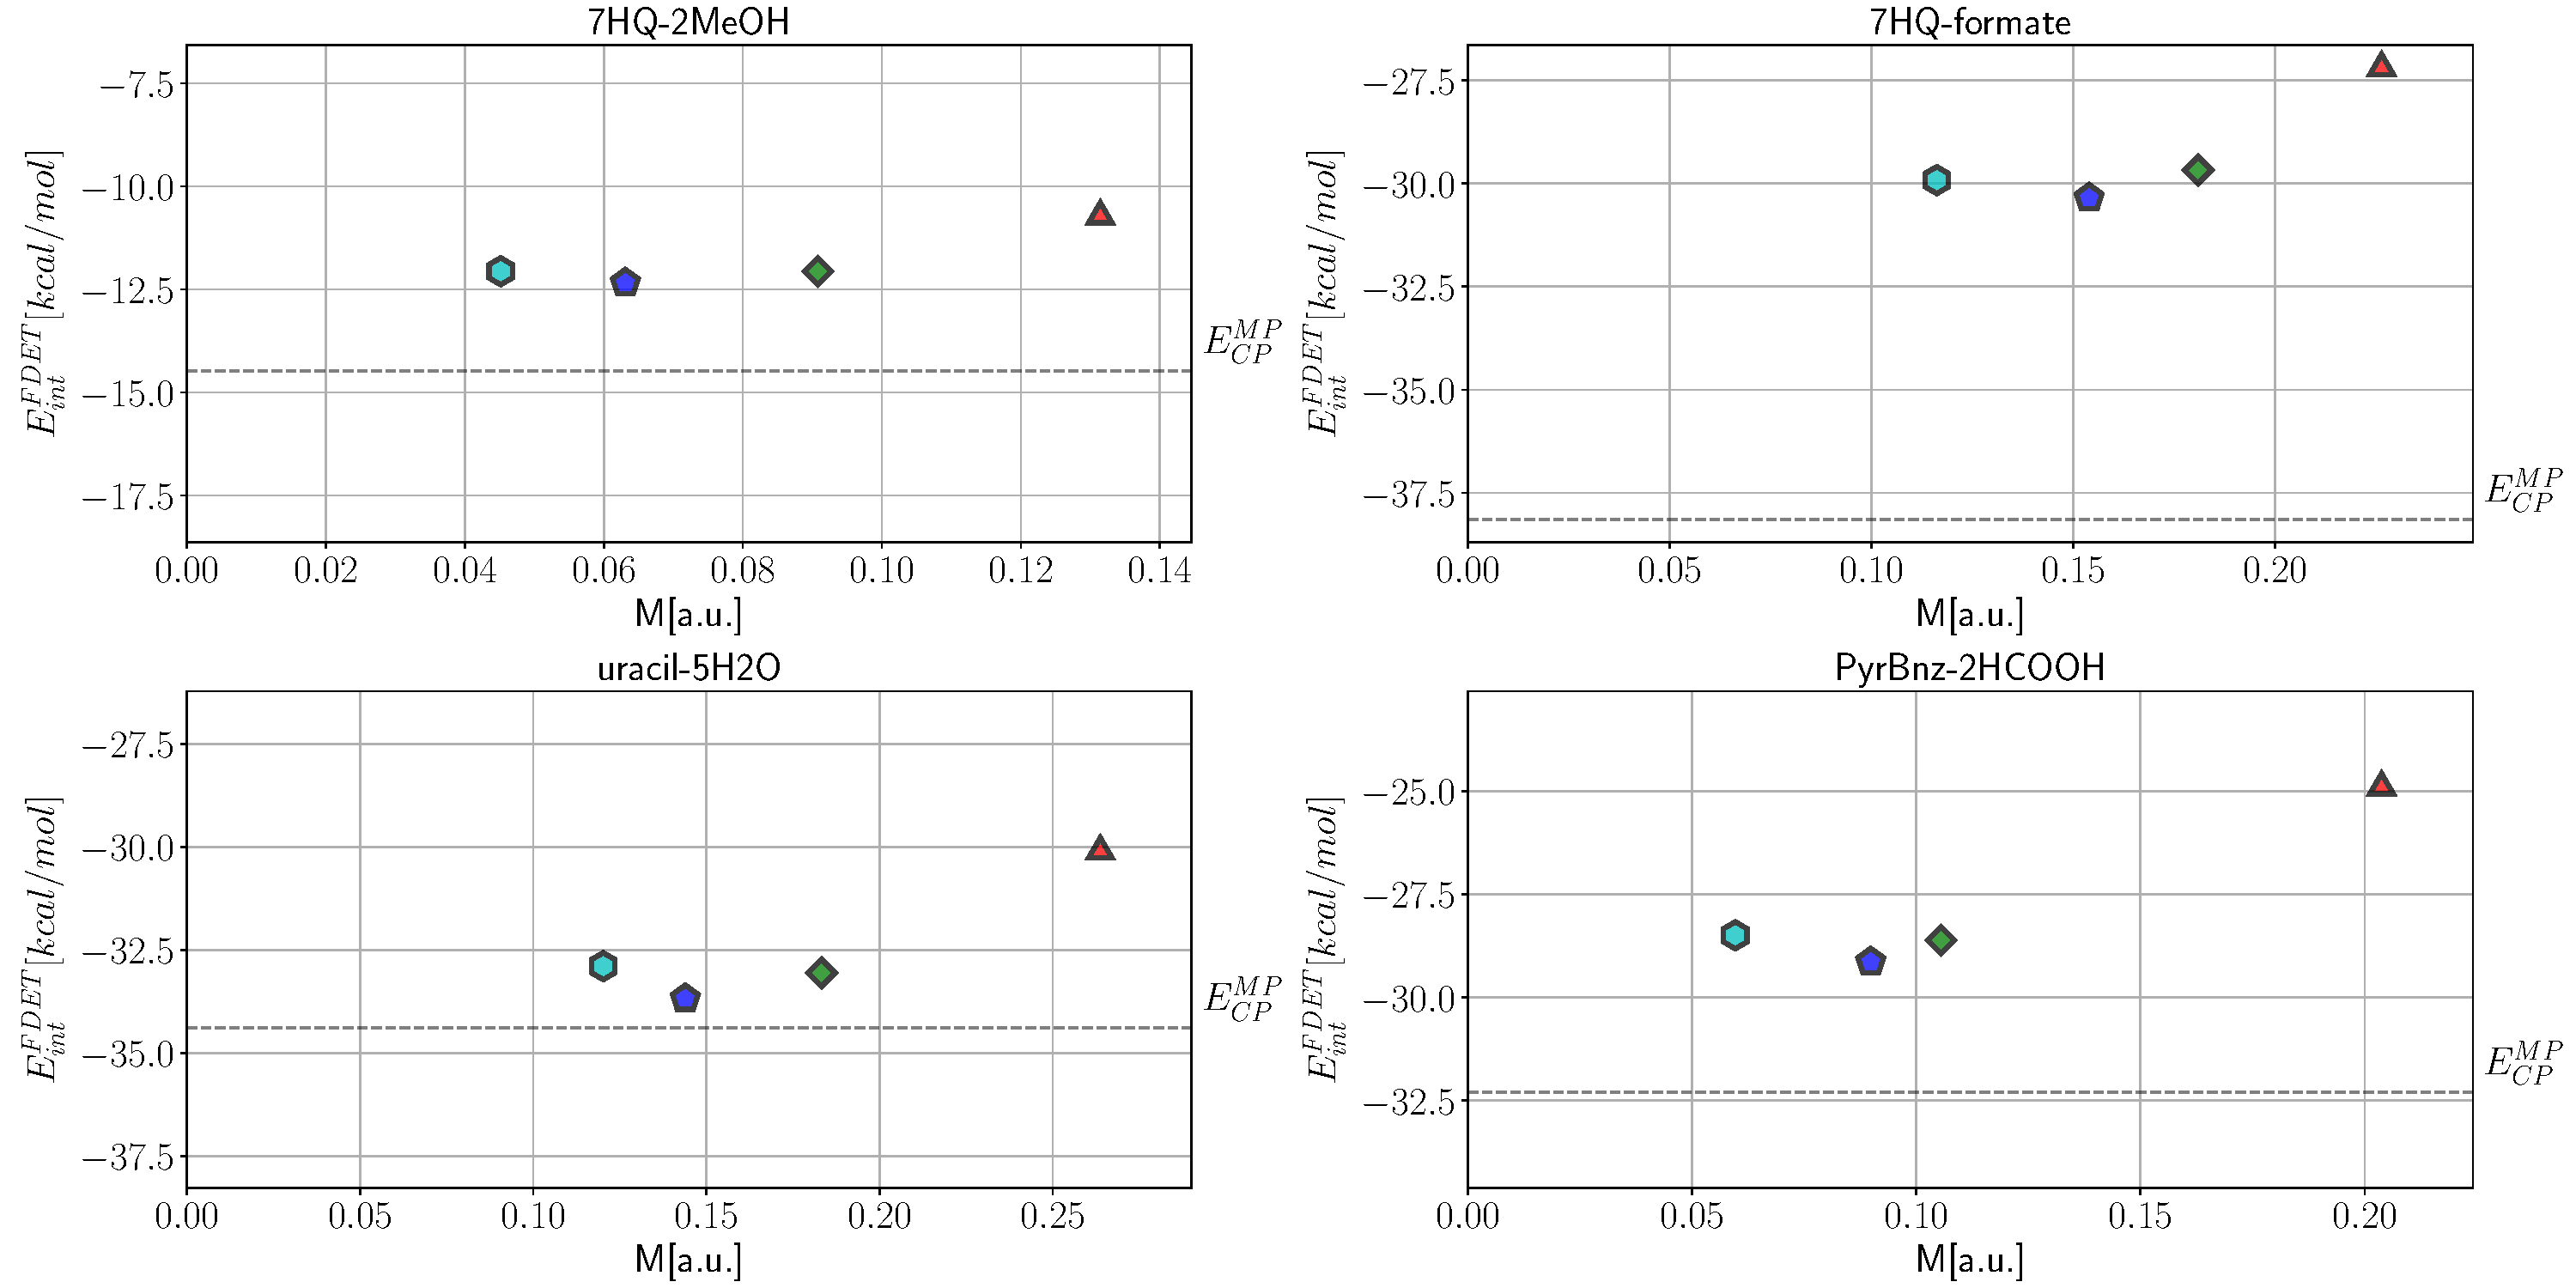
\includegraphics[width=1.0\linewidth]{M_vs_MP_ccpVDZ.pdf}
\caption{Integrated negative density $M$ and the FDET-MP2 interaction energy for various choices of $\rho_B$: a) $\rho_B^{isol}$ (orange triangles), b) $\rho_B^{FAT}$ (light blue hexagons), c) $\rho_B^{pp(Mulliken)}$ (green diamonds), and d) $\rho_B^{pp(ChelPG)}$ (dark blue pentagons). Data obtained using the {\it monomer expansion} and the cc-pVDZ basis set. Horizontal lies indicate the reference interaction energy.}
\label{fig:M_vs_MP_ccpVDZ}
\end{figure*}

\begin{figure*}
\centering
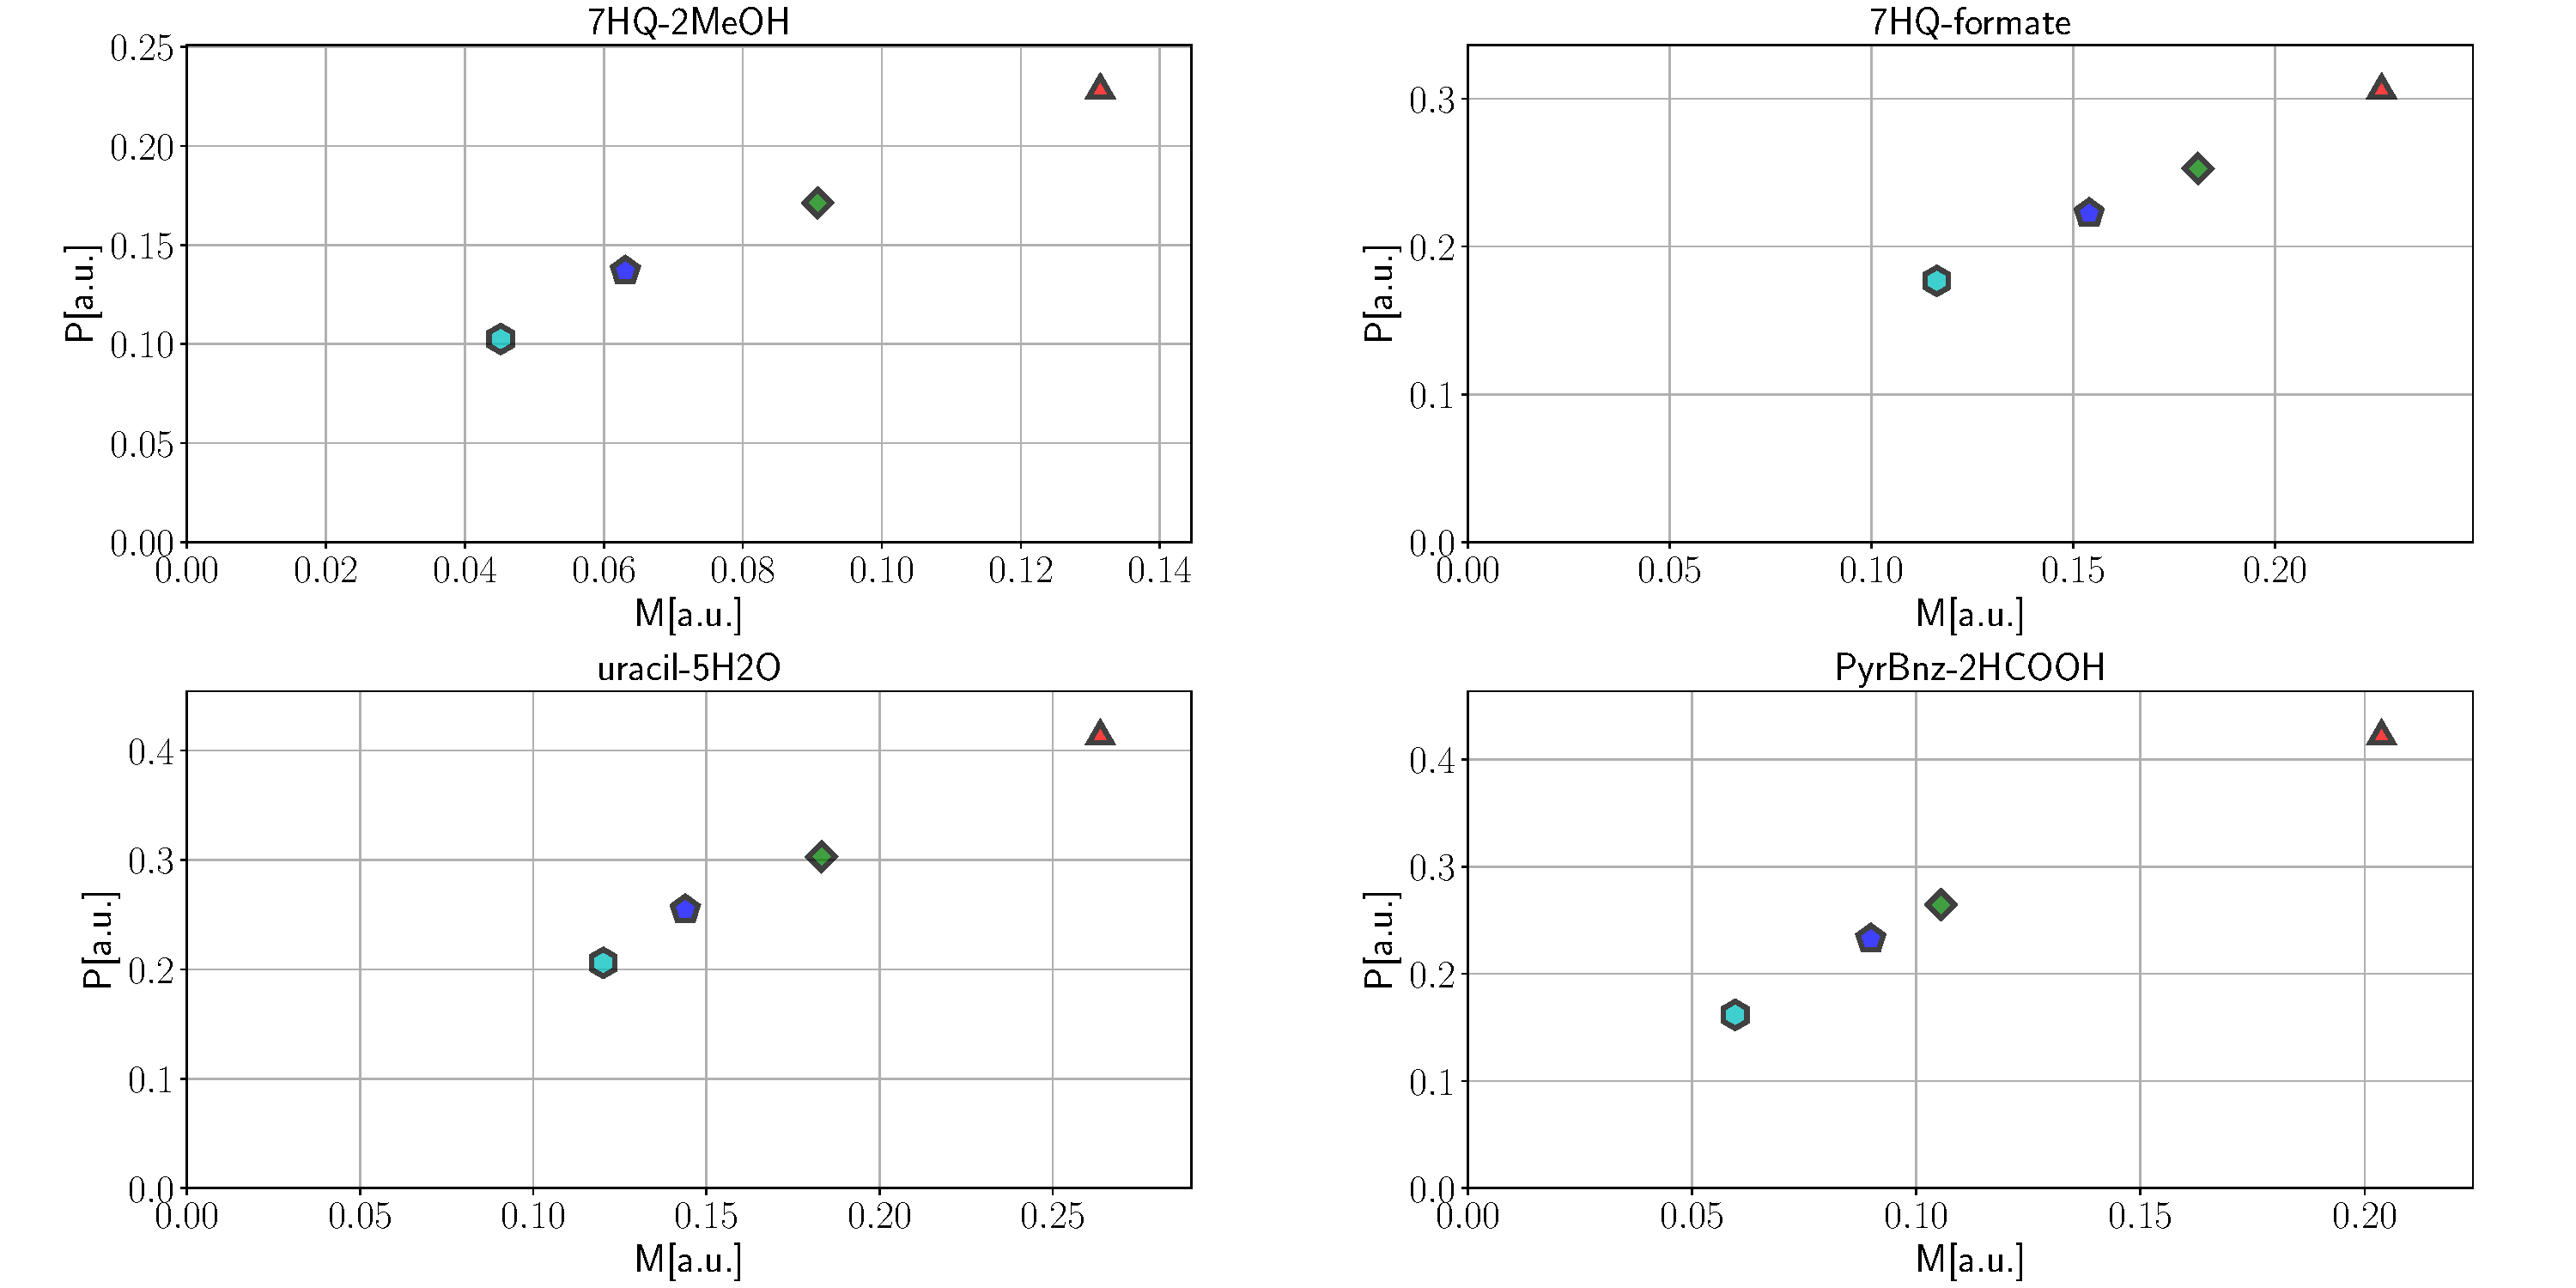
\includegraphics[width=1.0\linewidth]{M_vs_P_ccpVDZ.pdf}
\caption{Integrated negative density $M$ and the total density error $P$ for various choices of $\rho_B$: a) $\rho_B^{isol}$ (orange triangles), b) $\rho_B^{FAT}$ (light blue hexagons), c) $\rho_B^{pp(Mulliken)}$ (green diamonds), and d) $\rho_B^{pp(ChelPG)}$ (dark blue pentagons). Data obtained using the {\it monomer expansion} and the cc-pVDZ basis set.}
\label{fig:M_vs_P_ccpVDZ<}
\end{figure*}
\subsection{aug-cc-pVDZ}
\begin{table}[H]
\begin{center}
\resizebox{0.875\paperwidth}{!}{
\begin{tabular}{|l|l|l|l|l|l|l|l|l|l|}\hline
complex & $\rho_B$ & $E_k[\Delta \rho^{c}_{v'_A}, \rho'_A, \rho_B]$ $^{[a]}$ & $E_k[\Delta \rho^{c}_{v'_B}, \rho'_B, \rho_A]$ $^{[a]}$ & $E^{FDET(\rho_B)}_{int}$ $^{[b]}$ & $E_{int}^{ref}$ $^{[c]}$& $\Delta_{CP}$ $^{[d]}$ & $M$ $^{[e]}$ & $P$ $^{[f]}$ & $P_{cmpl}$ $^{[g]}$\\\hline
7HQ-2MeOH & $\rho_B^{isol}$ & 0.092 & × & -10.983 & -17.473 & 5.632& 0.121 & 0.228 & 0.362\\\hline
7HQ-2MeOH & $\rho_B^{FAT}$ & 0.081 & 0.127 & -14.269 & -17.473 & 5.632 & 0.007 & 0.059 & 0.362\\\hline
7HQ-formate & $\rho_B^{isol}$ & 0.020 & × & -23.037 & -36.485 & 3.522 & 0.206 & 0.316 & 0.670\\\hline
7HQ-formate & $\rho_B^{FAT}$ & -0.008 & 0.068 & -33.325 &-36.485 & 3.522 & 0.007 & 0.066 & 0.670\\\hline
uracil-5H$_2$O & $\rho_B^{isol}$ & 0.224 & × & -32.065 & -38.620 & 7.839 & 0.234 & 0.426 & 0.633\\\hline
uracil-5H$_2$O & $\rho_B^{FAT}$ & 0.204 & 0.236 & -39.695 & -38.620 & 7.839 & 0.014 & 0.114 & 0.633\\\hline
PyrBnz-2HCOOH & $\rho_B^{isol}$ & 0.160 & × & -26.948 & -36.532 & 7.318 & 0.184 & 0.416 & 0.600\\\hline
PyrBnz-2HCOOH & $\rho_B^{FAT}$ & 0.131 & 0.164 & -34.894 & -36.532 & 7.318 & 0.013 & 0.104 & 0.600\\\hline
\multicolumn{10}{c}{ } \\
\multicolumn{10}{p{1.0\textwidth}}{$^{[a]}$ defined in Eq.~\ref{M-eq:nkernel} in the manuscript}\\
\multicolumn{10}{p{1.0\textwidth}}{$^{[b]}$ defined in Eq.~\ref{M-eq:eint2}, and Eq.~\ref{M-eq:eint4} in the manuscript for $\rho_B^{isol}$ and $\rho_B^{FAT }$ respectively.}\\
\multicolumn{10}{p{1.0\textwidth}}{$^{[c]}$ Counterpoise corrected, i.e. $E_{int}^{ref} = E_{v}^{(AB)} - E_{v_A}^{(AB)} - E_{v_B}^{(AB)}$, where all values are obtained with MP2, the subscript denotes the subsystem, and the superscript denotes the centres involved in the basis set expansion.} \\
\multicolumn{10}{p{1.0\textwidth}}{$^{[d]}$ Counterpoise correction: $\Delta_{CP} = E_{v_A}^{(A)} + E_{v_B}^{(B)} - E_{v_A}^{(AB)} - E_{v_B}^{(AB)}$, where all values are obtained with MP2, the subscript denotes the subsystem, and the superscript denotes the centres involved in the basis set expansion.} \\
\multicolumn{10}{p{1.0\textwidth}}{$^{[e]}$ $M=M[\rho_v^{o(ref)} - \rho^{FDET(FAT)}_{B}]$ with $M[\rho]$ defined in Eq.~\ref{M-eq:M} in the manuscript}\\
\multicolumn{10}{p{1.0\textwidth}}{$^{[f]}$ $P_{cmpl}=P[\rho_A^{isol}+\rho_B^{isol} - \rho_v^{o(ref)}]$ (cf. Eq.~\ref{M-eq:p_cmpl}), with $P[\rho]$ defined in Eq.~\ref{M-eq:def_P} in the manuscript}\\
\multicolumn{10}{p{1.0\textwidth}}{$^{[g]}$ $P=P[\rho_v^{o(ref)} - \rho_{tot}^{FDET(FAT)}]$ with $P[\rho]$ defined in Eq.~\ref{M-eq:def_P} in the manuscript}\\
\multicolumn{10}{p{1.0\textwidth}}{$^{[h]}$ $E^{FDET(FAT)}_{int}$ is given in Eq.~\ref{M-eq:eint4} in the manuscript}\\
\end{tabular}
}
\end{center}
\caption{Supplementary data for results obtained with the \textit{supermolecular expansion} and the aug-cc-pVDZ basis set. Energies are given in kcal/mol and quantities related to electron densities are given in atomic units.}
\end{table}

\begin{table}[H]
\begin{center}
\resizebox{0.875\paperwidth}{!}{
\begin{tabular}{|l|l|l|l|l|l|l|l|l|l|}\hline
complex & $\rho_B$ & $E_k[\Delta \rho^{c}_{v'_A}, \rho'_A, \rho_B]$ $^{[a]}$ & $E_k[\Delta \rho^{c}_{v'_B}, \rho'_B, \rho_A]$ $^{[a]}$ & $E^{FDET(\rho_B)}_{int}$ $^{[b]}$ & $E_{int}^{ref}$ $^{[c]}$ & $\Delta_{CP}$ $^{[d]}$ & $M$ $^{[e]}$ & $P$ $^{[f]}$ & $P_{cmpl}$ $^{[g]}$\\\hline
7HQ-2MeOH & $\rho_B^{isol}$ & 0.087 & × & -10.702 & -17.473 & 5.632 & 0.123 & 0.231 & 0.368\\\hline
7HQ-2MeOH & $\rho_B^{pp(Mulliken)}$ & 0.084 & × & -10.688 & -17.473 & 5.632 & 0.121 & 0.221 & 0.368\\\hline
7HQ-2MeOH & $\rho_B^{pp(ChelPG)}$ & 0.084 & × & -13.492 & -17.473 & 5.632 & 0.037 & 0.118 & 0.368\\\hline
7HQ-2MeOH & $\rho_B^{FAT}$ & 0.081 & 0.128 & -13.181 & -17.473 & 5.632 & 0.013 & 0.073 & 0.368\\\hline
7HQ-formate & $\rho_B^{isol}$ & 0.021 & × & -22.927 & -36.485 & 3.522 & 0.205 & 0.316 & 0.673\\\hline
7HQ-formate & $\rho_B^{pp(Mulliken)}$ & 0.016 & × & -27.202 & -36.485 & 3.522 & 0.148 & 0.242 & 0.673\\\hline
7HQ-formate & $\rho_B^{pp(ChelPG)}$ & 0.015 & × & -28.678 & -36.485 & 3.522 & 0.096 & 0.186 & 0.673\\\hline
7HQ-formate & $\rho_B^{FAT}$ & 0.011 & 0.117 & -28.028 & -36.485 & 3.522 & 0.036 & 0.114 & 0.673\\\hline
uracil-5H$_2$O & $\rho_B^{isol}$ & 0.212 & × & -31.629 & -38.620 & 7.839 & 0.237 & 0.427 & 0.643\\\hline
uracil-5H$_2$O & $\rho_B^{pp(Mulliken)}$ & 0.201 & × & -35.221 & -38.620 & 7.839 & 0.173 & 0.305 & 0.643\\\hline
uracil-5H$_2$O & $\rho_B^{pp(ChelPG)}$ & 0.205 & × & -38.010 & -38.620 & 7.839 & 0.058 & 0.206 & 0.643\\\hline
uracil-5H$_2$O & $\rho_B^{FAT}$ & 0.196 & 0.234 & -37.182 & -38.620 & 7.839 & 0.024 & 0.129 & 0.643\\\hline
PyrBnz-2HCOOH & $\rho_B^{isol}$ & 0.161 & × & -25.795 & -36.532 & 7.318 & 0.185 & 0.419 & 0.606\\\hline
PyrBnz-2HCOOH & $\rho_B^{pp(Mulliken)}$ & 0.141 & × & -31.448 & -36.532 & 7.318 & 0.152 & 0.281 & 0.606\\\hline
PyrBnz-2HCOOH & $\rho_B^{pp(ChelPG)}$ & 0.146 & × & -32.291 & -36.532 & 7.318 & 0.057 & 0.215 & 0.606\\\hline
PyrBnz-2HCOOH & $\rho_B^{FAT}$ & 0.139 & 0.164 & -32.418 & -36.532 & 7.318 & 0.016 & 0.127 & 0.606\\\hline
\multicolumn{10}{c}{ } \\
\multicolumn{10}{p{1.0\textwidth}}{$^{[a]}$ defined in Eq.~\ref{M-eq:nkernel} in the manuscript}\\
\multicolumn{10}{p{1.0\textwidth}}{$^{[b]}$ defined in Eq.~\ref{M-eq:eint2}, and Eq.~\ref{M-eq:eint4} in the manuscript for $\rho_B^{isol}$ and $\rho_B^{FAT }$ respectively, and in Eq.~\ref{M-eq:eint3} for $\rho_B^{pp(Mulliken)}$ and $\rho_B^{pp(ChelPG)}$}\\
\multicolumn{10}{p{1.0\textwidth}}{$^{[c]}$ Counterpoise corrected, i.e. $E_{int}^{ref} = E_{v}^{(AB)} - E_{v_A}^{(AB)} - E_{v_B}^{(AB)}$, where all values are obtained with MP2, the subscript denotes the subsystem, and the superscript denotes the centres involved in the basis set expansion.} \\
\multicolumn{10}{p{1.0\textwidth}}{$^{[d]}$ Counterpoise correction: $\Delta_{CP} = E_{v_A}^{(A)} + E_{v_B}^{(B)} - E_{v_A}^{(AB)} - E_{v_B}^{(AB)}$, where all values are obtained with MP2, the subscript denotes the subsystem, and the superscript denotes the centres involved in the basis set expansion.} \\
\multicolumn{10}{p{1.0\textwidth}}{$^{[e]}$ $M=M[\rho_v^{o(ref)} - \rho^{FDET(FAT)}_{B}]$ with $M[\rho]$ defined in Eq.~\ref{M-eq:M} in the manuscript}\\
\multicolumn{10}{p{1.0\textwidth}}{$^{[f]}$ $P_{cmpl}=P[\rho_A^{isol}+\rho_B^{isol} - \rho_v^{o(ref)}]$ (cf. Eq.~\ref{M-eq:p_cmpl}), with $P[\rho]$ defined in Eq.~\ref{M-eq:def_P} in the manuscript}\\
\multicolumn{10}{p{1.0\textwidth}}{$^{[g]}$ $P=P[\rho_v^{o(ref)} - \rho_{tot}^{FDET(FAT)}]$ with $P[\rho]$ defined in Eq.~\ref{M-eq:def_P} in the manuscript}\\
\multicolumn{10}{p{1.0\textwidth}}{$^{[h]}$ $E^{FDET(FAT)}_{int}$ is given in Eq.~\ref{M-eq:eint4} in the manuscript}\\
\end{tabular}
}
\end{center}
\caption{Supplementary data for results obtained with the \textit{monomer expansion} and the aug-cc-pVDZ basis set. Energies are given in kcal/mol and quantities related to electron densities are given in atomic units.}
\end{table}

\subsection{cc-pVTZ}
\begin{table}[H]
\begin{center}
\resizebox{0.875\paperwidth}{!}{
\begin{tabular}{|l|l|l|l|l|l|l|l|l|l|}\hline
complex & $\rho_B$ & $E_k[\Delta \rho^{c}_{v'_A}, \rho'_A, \rho_B]$ $^{[a]}$ & $E_k[\Delta \rho^{c}_{v'_B}, \rho'_B, \rho_A]$ $^{[a]}$ & $E^{FDET(\rho_B)}_{int}$ $^{[b]}$ & $E_{int}^{ref}$ $^{[c]}$& $\Delta_{CP}$ $^{[d]}$ & $M$ $^{[e]}$ & $P$ $^{[f]}$ & $P_{cmpl}$ $^{[g]}$\\\hline
7HQ-2MeOH & $\rho_B^{isol}$ & 0.064 & × & -11.127 & -17.858 & 5.681 & 0.117 & 0.225 & 0.356\\\hline
7HQ-2MeOH & $\rho_B^{FAT}$ & 0.054 & 0.101 & -14.717 & -17.858 & 5.681 & 0.007 & 0.062 & 0.356\\\hline
7HQ-formate & $\rho_B^{isol}$ & 0.014 & × & -24.519 & -39.521 & 6.011 & 0.196 & 0.307 & 0.663\\\hline
7HQ-formate & $\rho_B^{FAT}$ & -0.002 & 0.062 & -35.289 & -39.521 & 6.011 & 0.007 & 0.069 & 0.663\\\hline
uracil-5H$_2$O & $\rho_B^{isol}$ & 0.174 & × & -32.777 & -40.078 & 11.802 & 0.222 & 0.415 & 0.619\\\hline
uracil-5H$_2$O & $\rho_B^{FAT}$ & 0.156 & 0.179 & -41.188 & -40.078 & 11.802 & 0.014 & 0.118 & 0.619\\\hline
\multicolumn{10}{c}{ } \\
\multicolumn{10}{p{1.0\textwidth}}{$^{[a]}$ defined in Eq.~\ref{M-eq:nkernel} in the manuscript}\\
\multicolumn{10}{p{1.0\textwidth}}{$^{[b]}$ defined in Eq.~\ref{M-eq:eint2}, and Eq.~\ref{M-eq:eint4} in the manuscript for $\rho_B^{isol}$ and $\rho_B^{FAT }$ respectively.}\\
\multicolumn{10}{p{1.0\textwidth}}{$^{[c]}$ Counterpoise corrected, i.e. $E_{int}^{ref} = E_{AB}^{(AB)} - E_{v_A}^{(AB)} - E_{v_B}^{(AB)}$, where all values are obtained with MP2, the subscript denotes the subsystem, and the superscript denotes the centres involved in the basis set expansion.} \\
\multicolumn{10}{p{1.0\textwidth}}{$^{[d]}$ Counterpoise correction: $\Delta_{CP} = E_{v_A}^{(A)} + E_{v_B}^{(B)} - E_{v_A}^{(AB)} - E_{v_B}^{(AB)}$, where all values are obtained with MP2, the subscript denotes the subsystem, and the superscript denotes the centres involved in the basis set expansion.} \\
\multicolumn{10}{p{1.0\textwidth}}{$^{[e]}$ $M=M[\rho_v^{o(ref)} - \rho^{FDET(FAT)}_{B}]$ with $M[\rho]$ defined in Eq.~\ref{M-eq:M} in the manuscript}\\
\multicolumn{10}{p{1.0\textwidth}}{$^{[f]}$ $P_{cmpl}=P[\rho_A^{isol}+\rho_B^{isol} - \rho_v^{o(ref)}]$ (cf. Eq.~\ref{M-eq:p_cmpl}), with $P[\rho]$ defined in Eq.~\ref{M-eq:def_P} in the manuscript}\\
\multicolumn{10}{p{1.0\textwidth}}{$^{[g]}$ $P=P[\rho_v^{o(ref)} - \rho_{tot}^{FDET(FAT)}]$ with $P[\rho]$ defined in Eq.~\ref{M-eq:def_P} in the manuscript}\\
\multicolumn{10}{p{1.0\textwidth}}{$^{[h]}$ $E^{FDET(FAT)}_{int}$ is given in Eq.~\ref{M-eq:eint4} in the manuscript}\\
\end{tabular}
}
\end{center}
\caption{Supplementary data for results obtained with the \textit{supermolecular expansion} and the cc-pVTZ basis set. Energies are given in kcal/mol and quantities related to electron densities are given in atomic units.}
\end{table}

\begin{table}[H]
\begin{center}
\resizebox{0.875\paperwidth}{!}{
\begin{tabular}{|l|l|l|l|l|l|l|l|l|l|}\hline
complex & $\rho_B$ & $E_k[\Delta \rho^{c}_{v'_A}, \rho'_A, \rho_B]$ $^{[a]}$ & $E_k[\Delta \rho^{c}_{v'_B}, \rho'_B, \rho_A]$ $^{[a]}$ & $E^{FDET(\rho_B)}_{int}$ $^{[b]}$ & $E_{int}^{ref}$ $^{[c]}$ & $\Delta_{CP}$ $^{[d]}$ & $M$ $^{[e]}$ & $P$ $^{[f]}$ & $P_{cmpl}$ $^{[g]}$\\\hline
7HQ-2MeOH & $\rho_B^{isol}$ & 0.040 & × & -10.716 & -17.858 & 5.681 & 0.125 & 0.226 & 0.358\\\hline
7HQ-2MeOH & $\rho_B^{pp(Mulliken)}$ & 0.038 & × & -12.684 & -17.858 & 5.681 & 0.071 & 0.153 & 0.358\\\hline
7HQ-2MeOH & $\rho_B^{pp(ChelPG)}$ & 0.037 & × & -13.254 & -17.858 & 5.681 & 0.045 & 0.119 & 0.358\\\hline
7HQ-2MeOH & $\rho_B^{FAT}$ & 0.035 & 0.068 & -13.132 & -17.858 & 5.681 & 0.021 & 0.074 & 0.358\\\hline
7HQ-formate & $\rho_B^{isol}$ & 0.002 & × & -25.786 & -39.521 & 6.011 & 0.214 & 0.310 & 0.661\\\hline
7HQ-formate & $\rho_B^{pp(Mulliken)}$ & 0.003 & × & -29.829 & -39.521 & 6.011 & 0.145 & 0.230 & 0.661\\\hline
7HQ-formate & $\rho_B^{pp(ChelPG)}$ & 0.003 & × & -30.768 & -39.521 & 6.011 & 0.116 & 0.196 & 0.661\\\hline
7HQ-formate & $\rho_B^{FAT}$ & 0.003 & 0.064 & -30.578 & -39.521 & 6.011 & 0.057 & 0.127 & 0.661\\\hline
uracil-5H$_2$O & $\rho_B^{isol}$ & 0.119 & × & -32.283 & -40.078 & 11.802 & 0.247 & 0.413 & 0.617\\\hline
uracil-5H$_2$O & $\rho_B^{pp(Mulliken)}$ & 0.112 & × & -37.341 & -40.078 & 11.802 & 0.123 & 0.249 & 0.617\\\hline
uracil-5H$_2$O & $\rho_B^{pp(ChelPG)}$ & 0.111 & × & -37.944 & -40.078 & 11.802 & 0.091 & 0.212 & 0.617\\\hline
uracil-5H$_2$O & $\rho_B^{FAT}$ & 0.104 & 0.099 & -37.489 & -40.078 & 11.802 & 0.054 & 0.139 & 0.617\\\hline
PyrBnz-2HCOOH & $\rho_B^{isol}$ & 0.117 & × & -25.481 & -37.236 & 7.135 & 0.192 & 0.416 & 0.594\\\hline
PyrBnz-2HCOOH & $\rho_B^{pp(Mulliken)}$ & 0.106 & × & -30.000 & -37.236 & 7.135 & 0.083 & 0.249 & 0.594\\\hline
PyrBnz-2HCOOH & $\rho_B^{pp(ChelPG)}$ & 0.101 & × & -31.343 & -37.236 & 7.135 & 0.067 & 0.209 & 0.594\\\hline
PyrBnz-2HCOOH & $\rho_B^{FAT}$ & 0.091 & 0.078 & -31.420 & -37.236 & 7.135 & 0.025 & 0.122 & 0.594\\\hline
\multicolumn{10}{c}{ } \\
\multicolumn{10}{p{1.0\textwidth}}{$^{[a]}$ defined in Eq.~\ref{M-eq:nkernel} in the manuscript}\\
\multicolumn{10}{p{1.0\textwidth}}{$^{[b]}$ defined in Eq.~\ref{M-eq:eint2}, and Eq.~\ref{M-eq:eint4} in the manuscript for $\rho_B^{isol}$ and $\rho_B^{FAT }$ respectively, and in Eq.~\ref{M-eq:eint3} for $\rho_B^{pp(Mulliken)}$ and $\rho_B^{pp(ChelPG)}$}\\
\multicolumn{10}{p{1.0\textwidth}}{$^{[c]}$ Counterpoise corrected, i.e. $E_{int}^{ref} = E_{v}^{(AB)} - E_{v_A}^{(AB)} - E_{v_B}^{(AB)}$, where all values are obtained with MP2, the subscript denotes the subsystem, and the superscript denotes the centres involved in the basis set expansion.} \\
\multicolumn{10}{p{1.0\textwidth}}{$^{[d]}$ Counterpoise correction: $\Delta_{CP} = E_{v_A}^{(A)} + E_{v_B}^{(B)} - E_{v_A}^{(AB)} - E_{v_B}^{(AB)}$, where all values are obtained with MP2, the subscript denotes the subsystem, and the superscript denotes the centres involved in the basis set expansion.} \\
\multicolumn{10}{p{1.0\textwidth}}{$^{[e]}$ $M=M[\rho_v^{o(ref)} - \rho^{FDET(FAT)}_{B}]$ with $M[\rho]$ defined in Eq.~\ref{M-eq:M} in the manuscript}\\
\multicolumn{10}{p{1.0\textwidth}}{$^{[f]}$ $P_{cmpl}=P[\rho_A^{isol}+\rho_B^{isol} - \rho_v^{o(ref)}]$ (cf. Eq.~\ref{M-eq:p_cmpl}), with $P[\rho]$ defined in Eq.~\ref{M-eq:def_P} in the manuscript}\\
\multicolumn{10}{p{1.0\textwidth}}{$^{[g]}$ $P=P[\rho_v^{o(ref)} - \rho_{tot}^{FDET(FAT)}]$ with $P[\rho]$ defined in Eq.~\ref{M-eq:def_P} in the manuscript}\\
\multicolumn{10}{p{1.0\textwidth}}{$^{[h]}$ $E^{FDET(FAT)}_{int}$ is given in Eq.~\ref{M-eq:eint4} in the manuscript}\\
\end{tabular}
}
\end{center}
\caption{Supplementary data for results obtained with the \textit{monomer expansion} and the cc-pVTZ basis set. Energies are given in kcal/mol and quantities related to electron densities are given in atomic units.}
\end{table}

\begin{figure*}
\centering
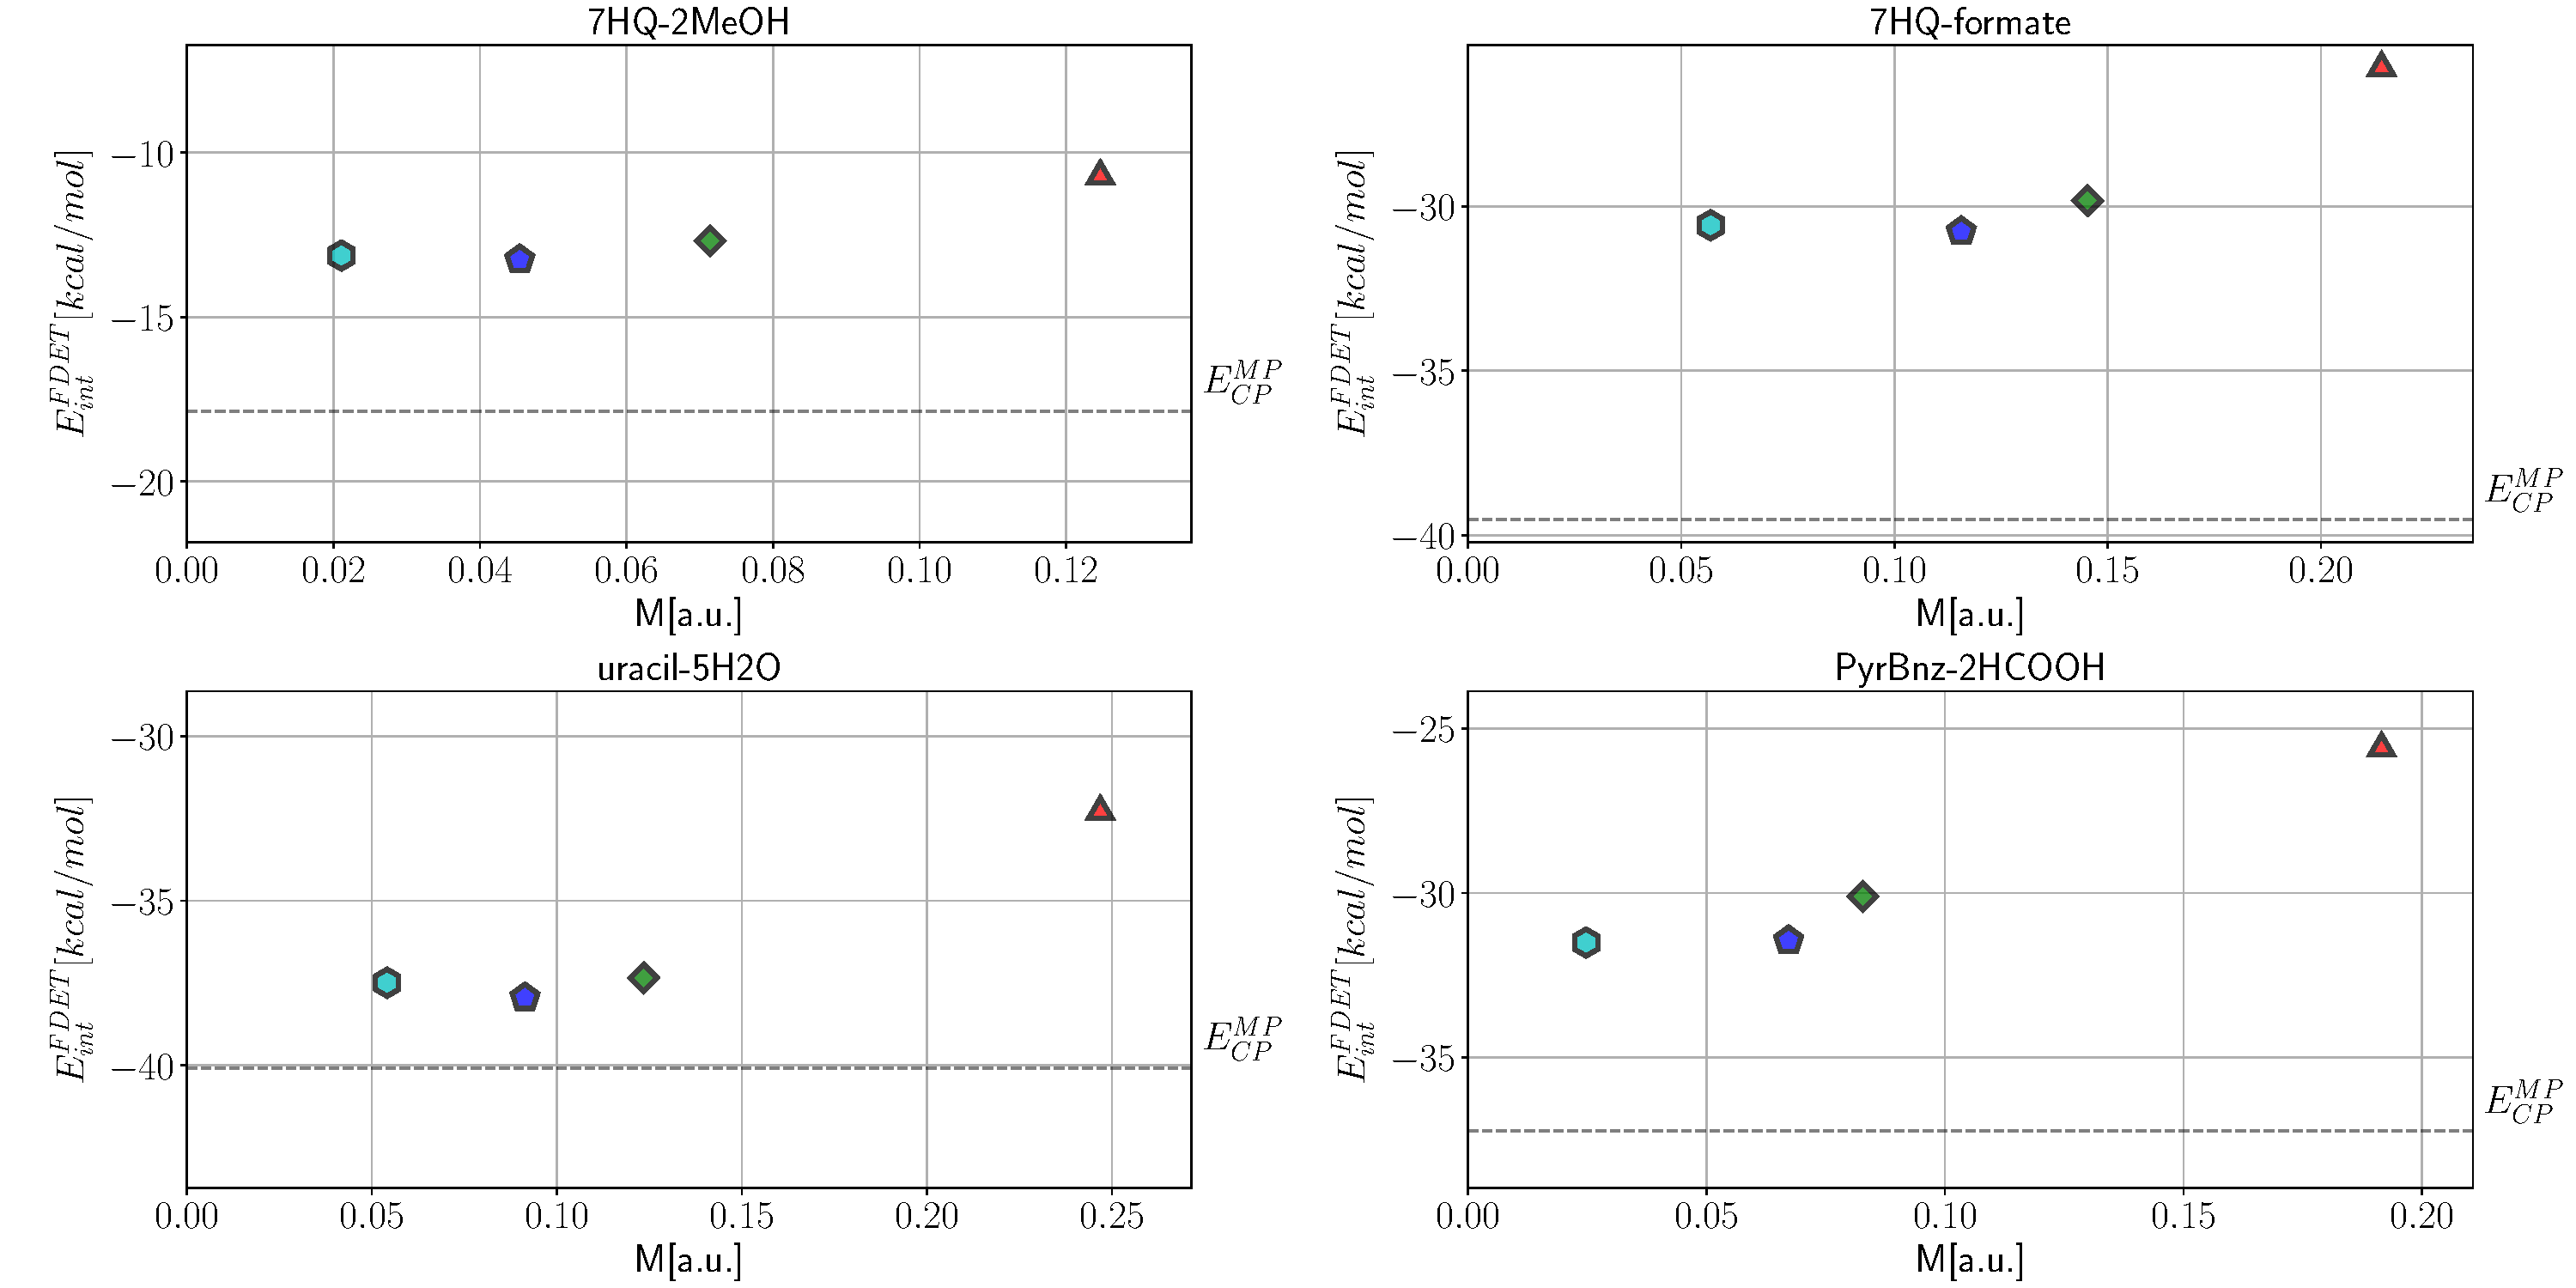
\includegraphics[width=1.0\linewidth]{M_vs_MP_ccpVTZ.pdf}
\caption{Integrated negative density $M$ and the FDET-MP2 interaction energy for various choices of $\rho_B$: a) $\rho_B^{isol}$ (orange triangles), b) $\rho_B^{FAT}$ (light blue hexagons), c) $\rho_B^{pp(Mulliken)}$ (green diamonds), and d) $\rho_B^{pp(ChelPG)}$ (dark blue pentagons). Data obtained using the {\it monomer expansion} and the cc-pVTZ basis set. Horizontal lies indicate the reference interaction energy.}
\label{fig:M_vs_MP_ccpVTZ}
\end{figure*}

\begin{figure*}
\centering
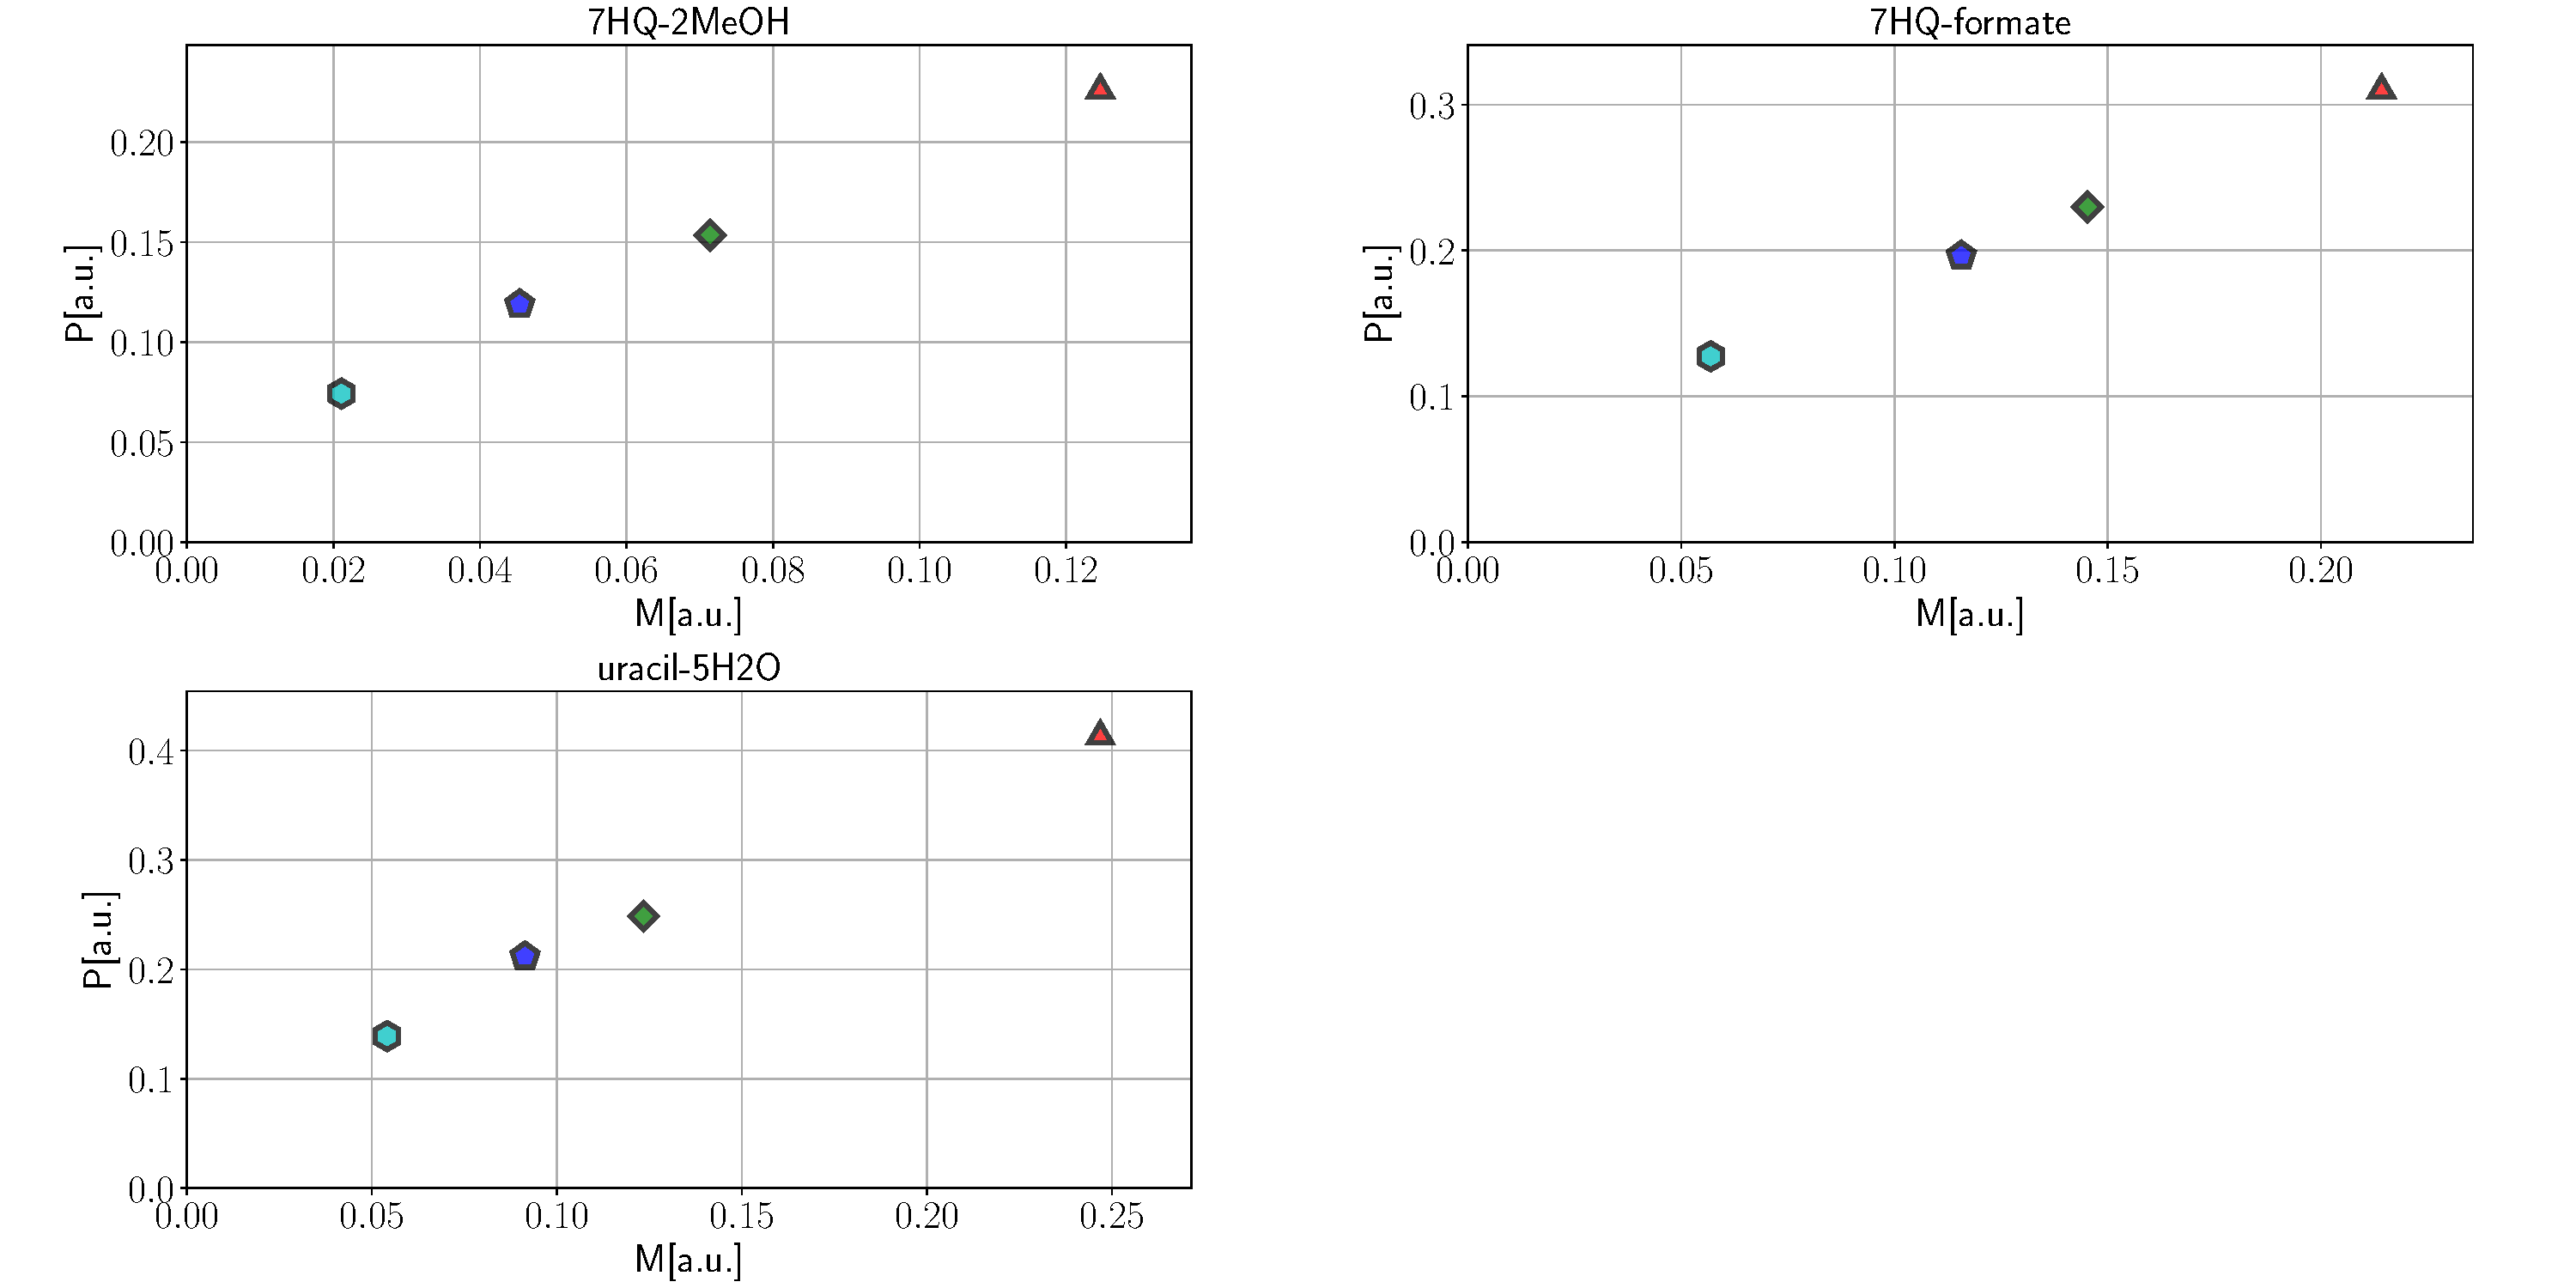
\includegraphics[width=1.0\linewidth]{M_vs_P_ccpVTZ.pdf}
\caption{Integrated negative density $M$ and the total density error $P$ for various choices of $\rho_B$: a) $\rho_B^{isol}$ (orange triangles), b) $\rho_B^{FAT}$ (light blue hexagons), c) $\rho_B^{pp(Mulliken)}$ (green diamonds), and d) $\rho_B^{pp(ChelPG)}$ (dark blue pentagons). Data obtained using the {\it monomer expansion} and the cc-pVTZ basis set.}
\label{fig:M_vs_P_ccpVTZ}
\end{figure*}

\subsection{aug-cc-pVTZ}
\begin{table}[H]
\begin{center}
\resizebox{0.875\paperwidth}{!}{
\begin{tabular}{|l|l|l|l|l|l|l|l|l|l|}\hline
complex & $\rho_B$ & $E_k[\Delta \rho^{c}_{v'_A}, \rho'_A, \rho_B]$ $^{[a]}$ & $E_k[\Delta \rho^{c}_{v'_B}, \rho'_B, \rho_A]$ $^{[a]}$ & $E^{FDET(\rho_B)}_{int}$ $^{[b]}$ & $E_{int}^{ref}$ $^{[c]}$ & $\Delta_{CP}$ $^{[d]}$ & $M$ $^{[e]}$ & $P$ $^{[f]}$ & $P_{cmpl}$ $^{[g]}$\\\hline
uracil-5H$_2$O & $\rho_B^{isol}$ & 0.000303 & × & -31.994 & -41.753 & 7.450 & 0.230 & 0.426 & 0.630\\\hline
uracil-5H$_2$O & $\rho_B^{pp(Mulliken)}$ & 0.000286 & × & -39.046 & -41.753 & 7.450 & 0.087 & 0.218 & 0.630\\\hline
uracil-5H$_2$O & $\rho_B^{pp(ChelPG)}$ & 0.000293 & × & -39.444 & -41.753 & 7.450 & 0.053 & 0.209 & 0.630\\\hline
uracil-5H$_2$O & $\rho_B^{FAT}$ & 0.000276 & 0.000324 & -39.061 & -41.753 & 7.450 & 0.016 & 0.128 & 0.630\\\hline
\multicolumn{10}{c}{ } \\
\multicolumn{10}{p{1.0\textwidth}}{$^{[a]}$ defined in Eq.~\ref{M-eq:nkernel} in the manuscript}\\
\multicolumn{10}{p{1.0\textwidth}}{$^{[b]}$ defined in Eq.~\ref{M-eq:eint2}, and Eq.~\ref{M-eq:eint4} in the manuscript for $\rho_B^{isol}$ and $\rho_B^{FAT }$ respectively, and in Eq.~\ref{M-eq:eint3} for $\rho_B^{pp(Mulliken)}$ and $\rho_B^{pp(ChelPG)}$}\\
\multicolumn{10}{p{1.0\textwidth}}{$^{[c]}$ Counterpoise corrected, i.e. $E_{int}^{ref} = E_{v}^{(AB)} - E_{v_A}^{(AB)} - E_{v_B}^{(AB)}$, where all values are obtained with MP2, the subscript denotes the subsystem, and the superscript denotes the centres involved in the basis set expansion.} \\
\multicolumn{10}{p{1.0\textwidth}}{$^{[d]}$ Counterpoise correction: $\Delta_{CP} = E_{v_A}^{(A)} + E_{v_B}^{(B)} - E_{v_A}^{(AB)} - E_{v_B}^{(AB)}$, where all values are obtained with MP2, the subscript denotes the subsystem, and the superscript denotes the centres involved in the basis set expansion.} \\
\multicolumn{10}{p{1.0\textwidth}}{$^{[e]}$ $M=M[\rho_v^{o(ref)} - \rho^{FDET(FAT)}_{B}]$ with $M[\rho]$ defined in Eq.~\ref{M-eq:M} in the manuscript}\\
\multicolumn{10}{p{1.0\textwidth}}{$^{[f]}$ $P_{cmpl}=P[\rho_A^{isol}+\rho_B^{isol} - \rho_v^{o(ref)}]$ (cf. Eq.~\ref{M-eq:p_cmpl}), with $P[\rho]$ defined in Eq.~\ref{M-eq:def_P} in the manuscript}\\
\multicolumn{10}{p{1.0\textwidth}}{$^{[g]}$ $P=P[\rho_v^{o(ref)} - \rho_{tot}^{FDET(FAT)}]$ with $P[\rho]$ defined in Eq.~\ref{M-eq:def_P} in the manuscript}\\
\multicolumn{10}{p{1.0\textwidth}}{$^{[h]}$ $E^{FDET(FAT)}_{int}$ is given in Eq.~\ref{M-eq:eint4} in the manuscript}\\
\end{tabular}
}
\end{center}
\caption{Supplementary data for results obtained with the \textit{monomer expansion} and the aug-cc-pVTZ basis set. Energies are given in kcal/mol and quantities related to electron densities are given in atomic units.}
\end{table}

\begin{figure*}
\centering
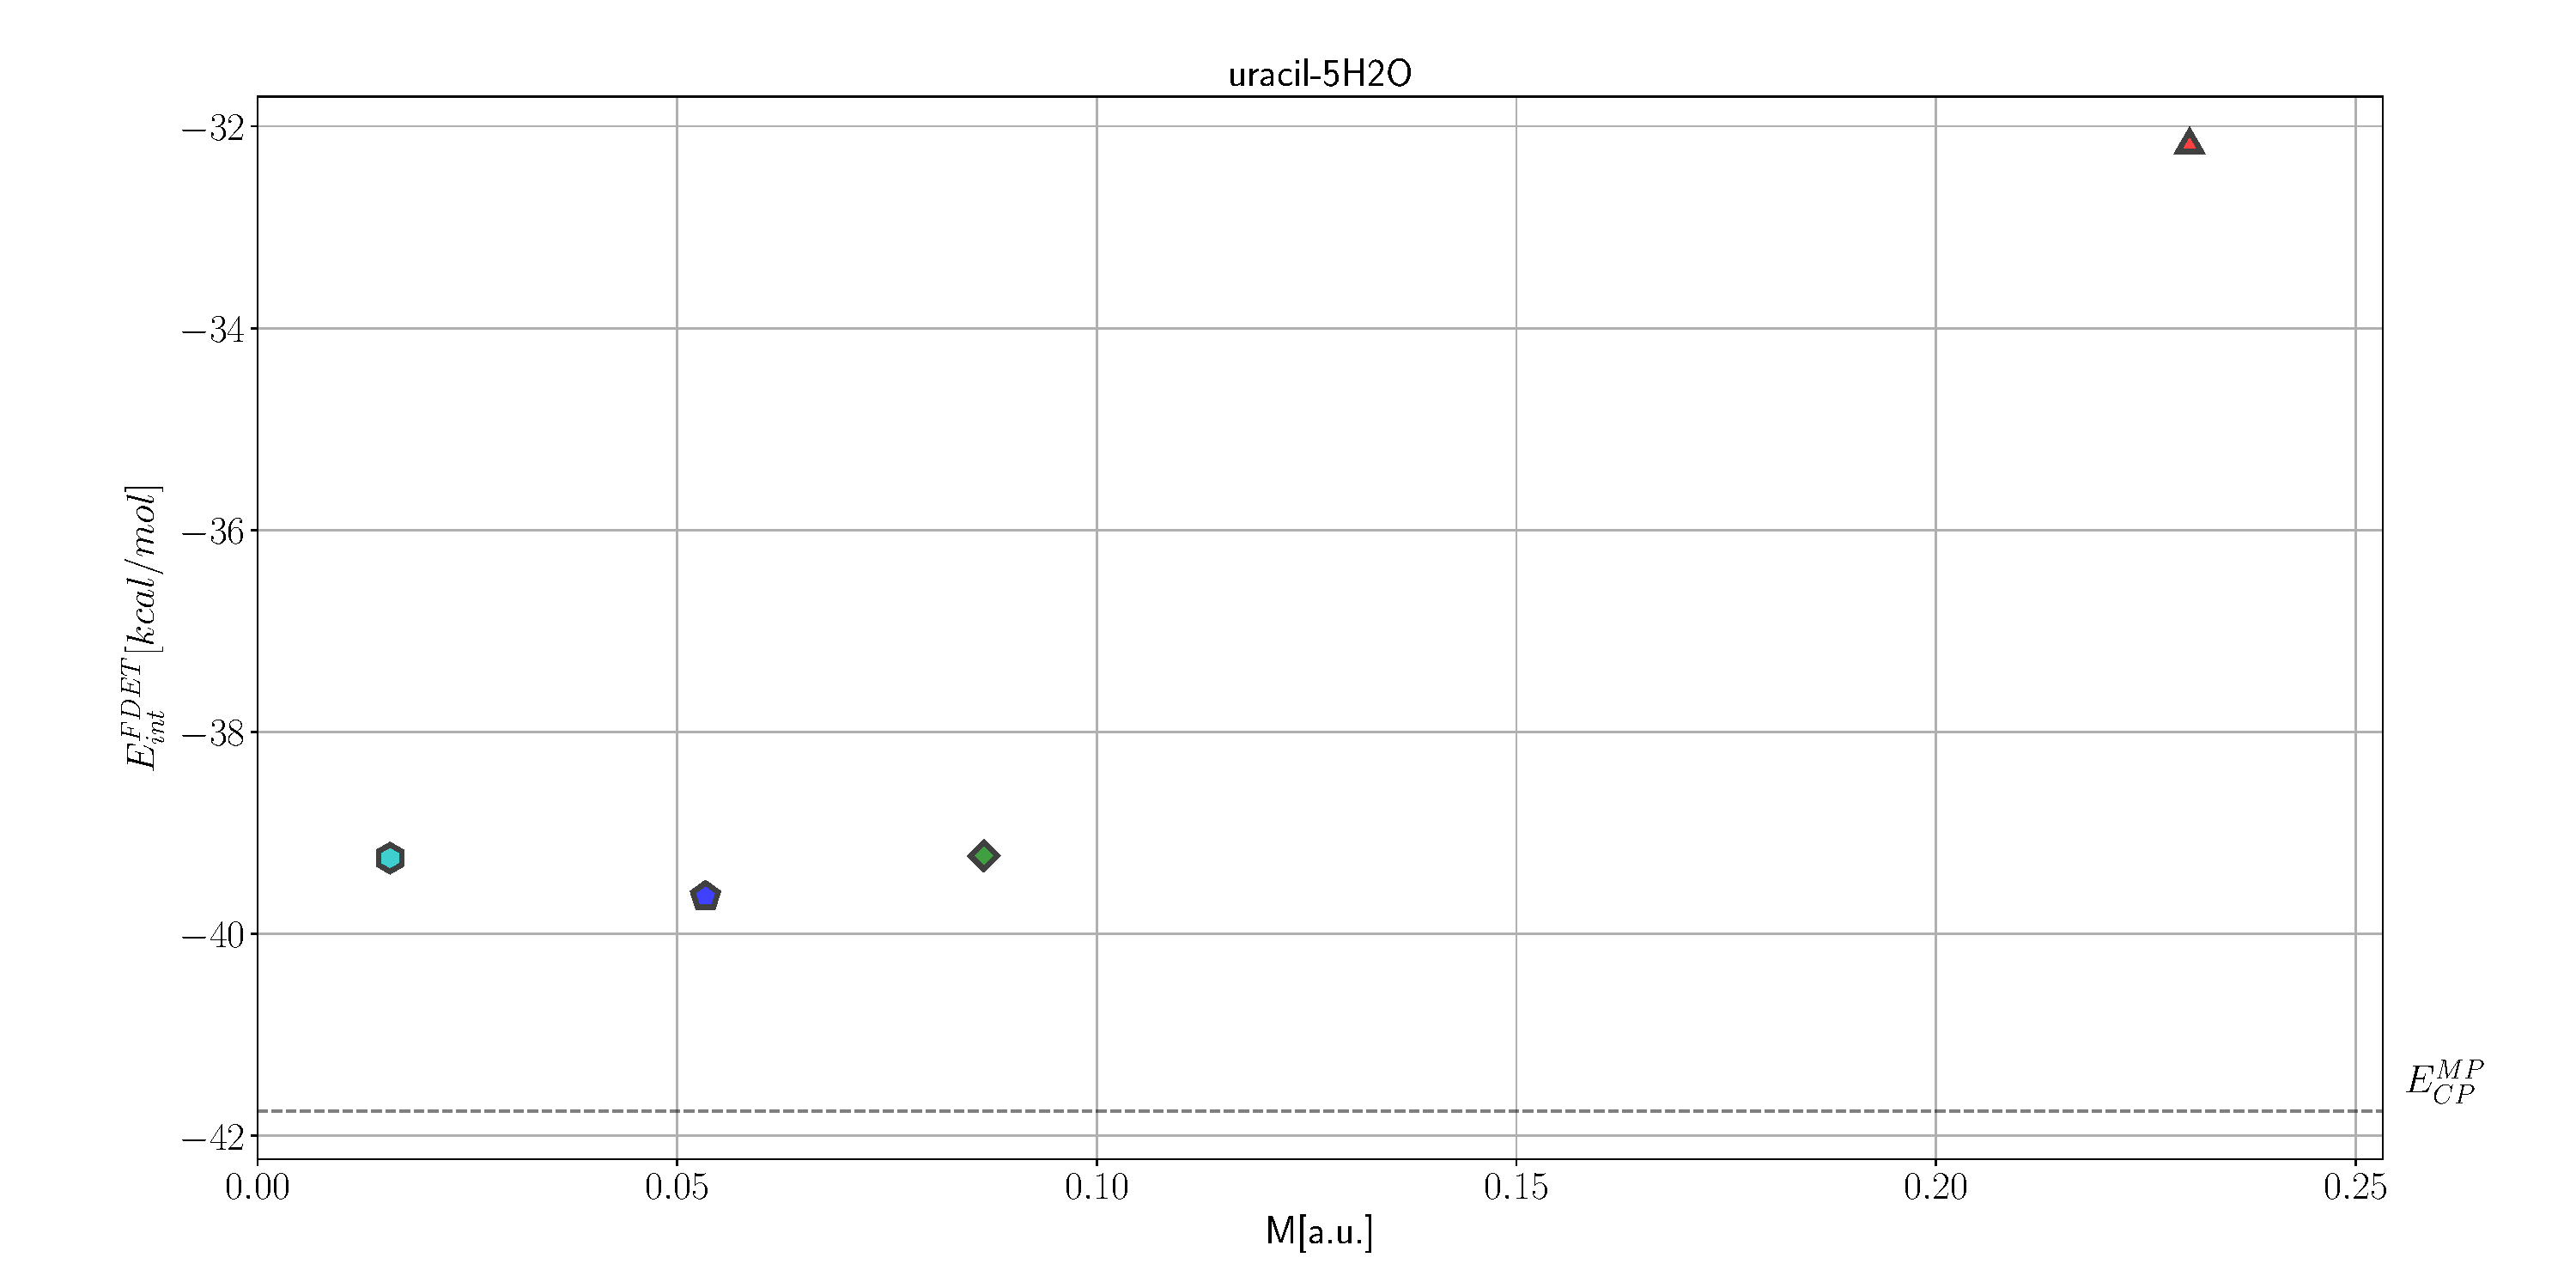
\includegraphics[width=1.0\linewidth]{M_vs_MP_augccpVTZ.pdf}
\caption{Integrated negative density $M$ and the FDET-MP2 interaction energy for various choices of $\rho_B$: a) $\rho_B^{isol}$ (orange triangles), b) $\rho_B^{FAT}$ (light blue hexagons), c) $\rho_B^{pp(Mulliken)}$ (green diamonds), and d) $\rho_B^{pp(ChelPG)}$ (dark blue pentagons). Data obtained using the {\it monomer expansion} and the aug-cc-pVTZ basis set. Horizontal lies indicate the reference interaction energy.}
\label{fig:M_vs_MP_augccpVTZ}
\end{figure*}

\begin{figure*}
\centering
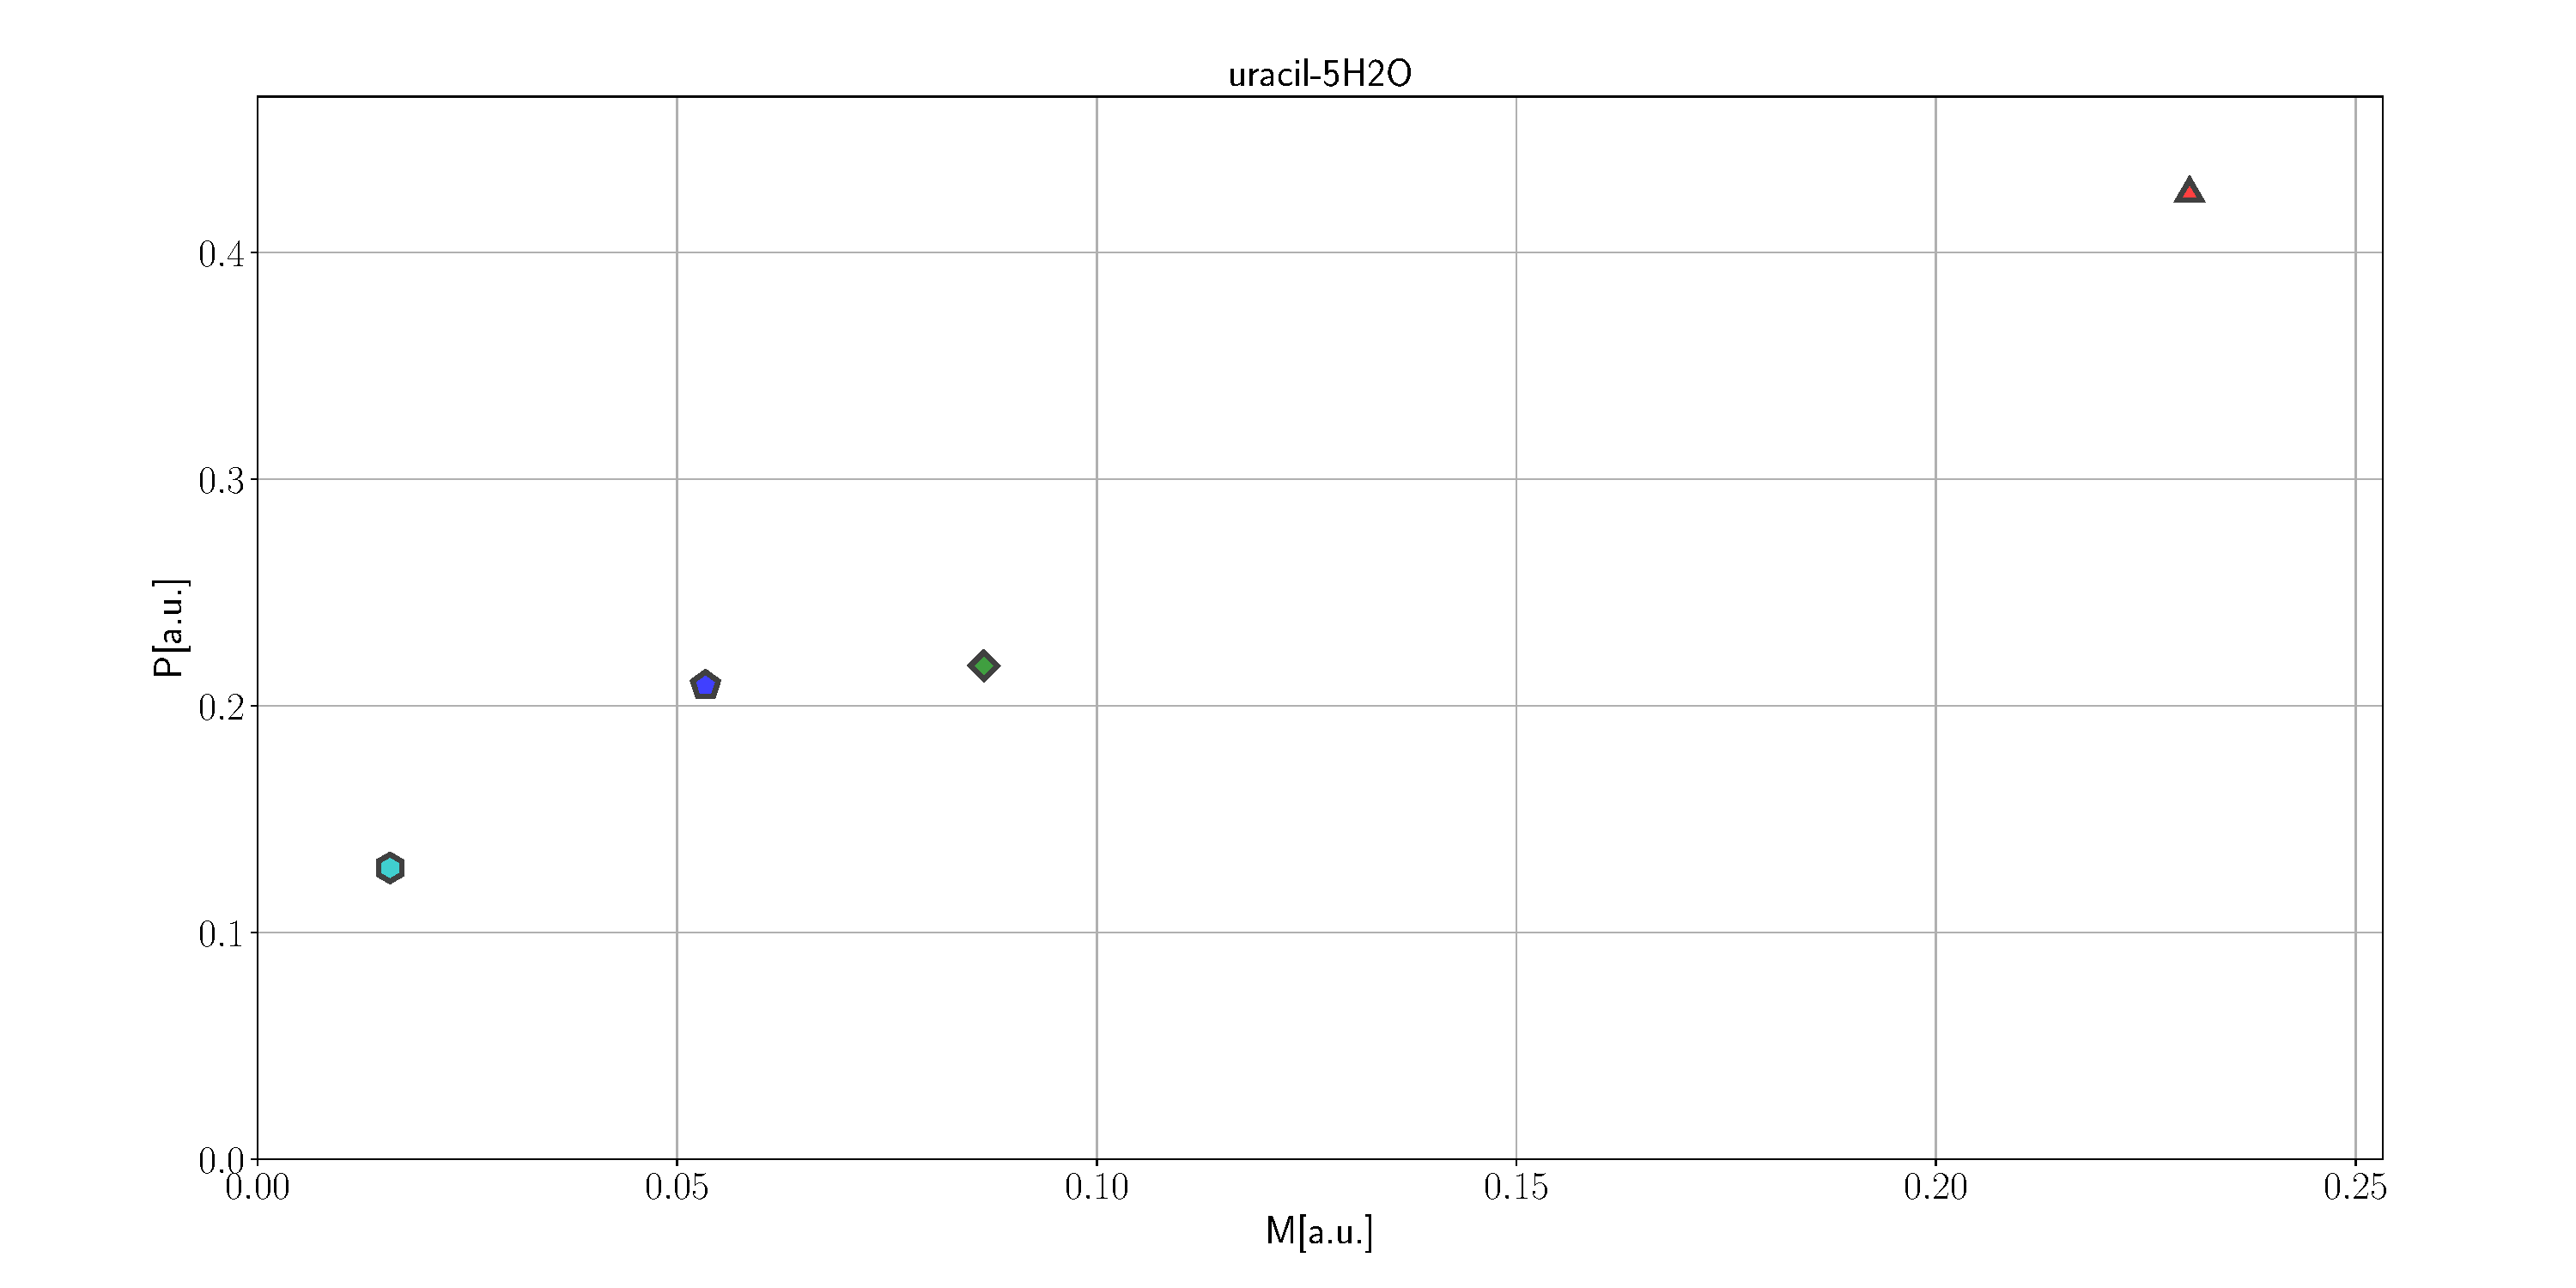
\includegraphics[width=1.0\linewidth]{M_vs_P_augccpVTZ.pdf}
\caption{Integrated negative density $M$ and the total density error $P$ for various choices of $\rho_B$: a) $\rho_B^{isol}$ (orange triangles), b) $\rho_B^{FAT}$ (light blue hexagons), c) $\rho_B^{pp(Mulliken)}$ (green diamonds), and d) $\rho_B^{pp(ChelPG)}$ (dark blue pentagons). Data obtained using the {\it monomer expansion} and the aug-cc-pVTZ basis set.}
\label{fig:M_vs_P_augccpVTZ}
\end{figure*}

\end{document}
